\chapter{Элементы физики сверхпроводящих квантовых цепей} \label{c1}

В Главе \ref{c1} кратко излагаются элементы физики сверхпроводимости, СКЦ и квантовой оптики, необходимые для изложения и обсуждения результатов диссертационной работы. Вначале кратко описываются причины возникновения сверхпроводимости и изгалаются основные физические свойства сверхпроводника. Затем подробно рассматривается эффект Джозефсона в туннельном SIS-переходе, описываются основные модели описания эффекта Джозефсона приводятся основные свойства такого SIS-перехода (далее называемого джозефсоновским переходом) в различных режимах работы. Делается вывод о том, почему джозефсоновский переход находит широкое применение в классической и квантовой сверхпроводящей электронике. Описывается общий формализм квантования сверхпроводящей электрической цепи и рассчитываются параметры некоторых видов СКЦ --- потоковый кубит, трансмон, а также rf-SQUID. 
Отдельный раздел посвящен элементам квантовой оптики --- науки, которая описывает квантование электромагнитного поля и эффекты взаимодействия такого поля с атомами и молекулами. 
\section{Обзор явления сверхпроводимости} \label{s1_sc_phys}
Явление сверхпроводимости было открыто в 1911 г. в лаборатории Х. Камерлинг-Оннеса, и практически сразу началось интенсивное как теоретическое, так и экспериментальное изучение данного явления. Оказалось, что некоторые металлы при температурах $T<T_c$ демонстрируют целый ряд необычных физических свойств. Опуская подробности, перечислим наиболее интересные свойства сверхпроводников:
\begin{enumerate}
	\item Полное отсутствие сопротивления электрическому току;
	\item Полное вытеснение магнитного поля из объема сверхпроводника (эффект Мейсснера);
	\item Квантование магнитного потока через замкнутый контур из сверхпроводящего металла;
	\item Скачкообразное возрастание теплоемкости металла при переходе через $T_c$.
\end{enumerate}	
Объяснить поведение сверхпроводников на феноменологическом уровне удалось с помощью классической теории Лондонов, которая опирается на двухжидкостную модель электронов в металле: часть электронов предполагаются <<сверхпроводящими>>, т.е. способными переносить электрический ток в отсутствие внешнего электрического поля. Одного этого предположения практически достаточно для того, чтоб объяснить многие свойства сверхпроводников, в частности, идеальный диамагнетизм. Квантовое обобщение этой теории было построено Гинзбургом и Ландау на основе теории фазовых переходов II рода. Ключевым предположением теории ГЛ было введение общей волновой функции сверхпроводящих электронов $\Psi = |\Psi(\mathbf{r})| e^{i\varphi({\mathbf{r}})}$ в металле и её рассмотрение в качестве параметра порядка, характеризующего фазовый переход. Некоторые вопросы, на которые теория Лондонов давала качественно неправильный ответ (например, значение поверхностной энергии границы между нормальной и сверхпроводящей фазами), были верно описаны с помощью теории ГЛ. Строго говоря, эта теория применима для описания сверхпроводимости в случае $T_c-T \ll T_c$\footnote[1]{Имеется также ограничение применимости теории, связанное с тем, что при $T$ очень близком к $T_c$ становятся важными флуктуационные эффекты.}, но оказывается, что для многих практически важных задач решение на основе теории ГЛ качественно совпадает с выводами микроскопической теории сверхпроводимости.

Несмотря на значительный прогресс в объяснении многих эксперименальных свойств сверхпроводников, истинный механизм возникновения сверхпроводимости долгое время оставался неописанным. Одним из результатов, указавшим на причину сверхпроводимости, стал изотопический эффект: для различных изотопов сверхпроводника в эксперименте наблюдается соотношение $T_c \cdot M^{\alpha}=\text{const}$. Следовательно, сверхпроводимость возникает из-за взаимодействия электронов с кристаллической решеткой. При детальном теоретическом анализе было выявлено, что возможен процесс эффективного притяжения электронов друг к другу посредством обмена фононами. В 1957 Купер \cite{CooperPairs} показал, что даже малое отрицательное (притягивающее) взаимодействие между электронами дает очень необычный результат. Состояние металла, в котором все электроны занимают состояния с $E<E_F$, даже при $T=0$ не является основным. В металле могут возникать определенного рода парные возбуждения, при которых два электрона с противоположными квазиимпульсами и спинами занимают состояния с энергией $E\approx E_F\! +\! \Delta$, где $\Delta$ --- некоторая константа, зависящая от температуры. Такие возбуждения называются \textit{куперовскими парами}, и их образование оказывается энергетически выгодным.  В 1958 г. Бардин, Купер и Шриффер \cite{Bardeen} нашли явный вид волновой функции основного состояния  и посчитали его энергию. Оказалось, что полная энергия состояния с некоторым количеством куперовских пар оказывается меньше по сравнению с энергией состояния металла без пар, на величину порядка $N(0)\Delta^2$. Параметр $\Delta$ определяется характером электрон-фононного взаимодействия. Его значение определяет критическую температуру: $\Delta = 1.76 k_b T_c$, среднее количество куперовских пар в металле: $\Delta N(0) \approx k_b T_c/E_F$, и кроме того, является средней энергей связи в паре в расчете на один электрон. По этой причине $\Delta$ называется \textit{энергетической щелью}: для разрыва куперовской пары необходимо затратить энергию $2\Delta$, при этом пара распадается на два квазичастичных возбуждения. Волновую функцию основного состояния пар в БКШ-теории можно записать как \cite{Tinkham}:
\begin{equation}
\ket{\psi_\varphi} = \prod_{\vec{k}}^{}(|u_{\vec{k}}|+|\nu_{\vec{k}}|e^{i\varphi}c^\dag_{\vec{k},\uparrow}c^\dagger_{-\vec{k}, \downarrow})\ket{\phi_0}.
\end{equation}  
Чрезвычайно важным обстоятельством является наличие фазового множителя при амплитуде вероятности рождения куперовской пары $|\nu_{\vec{k}}|$. Фаза $\varphi$ одна и та же для каждой пары и это иллюстрирует тот факт, что спаренные электроны образуют единое квантовое состояние. Для объемного и однородного сверхпроводника эта фаза не зависит от координаты. Можно показать, что в состоянии $\ket{\psi_\varphi}$ полное число пар не определено, однако, относительная дисперсия стремится к нулю по мере увеличения среднего числа электронов в системе, поэтому такое приближение можно считать разумным. Из состояний с $\ket{\psi_\varphi}$ c различными фазами можно получить состояние с определённым числом куперовских пар $\ket{\psi_n}$. Для этого достаточно заметить, что слагаемые в состояние $\ket{\psi_\varphi}$, отвечающие числу пар $N$ имеют фазовый множитель $e^{in{\varphi}}$, и при усреднении по фазам все остальные слагаемые дадут нулевой вклад:
\begin{equation}
\ket{\psi_n} = \int_{0}^{2 \pi}e^{-i n \varphi} \ket{\psi_\varphi}.
\end{equation} 
Соотношение между $\ket{\psi_\varphi}$ и $\ket{\psi_n}$ имеет такой же вид, как и для векторов состояния $\ket{x}$~и~$\ket{p}$ свободной частицы, то есть, $n$ и $\varphi$ в сверхпроводнике являются канонически сопряженными переменными. Для них можно вывести коммутационное соотношение $[\hat{n}, \hat{\varphi}]=-i$ и соотношение неопределенностей $\Delta\varphi \cdot \Delta n \approx \hbar$. Таким образом, изолированный остров сверхпроводника обладает макроскопической квантовой степенью свободы: фаза играет роль координаты, а число куперовских пар --- роль импульса. Ясно, что если остров находится при $T\!=\!0$ и полностью изолирован от других островов, то $N$ фиксировано, а значит $\phi$ полностью неопределена и не имеет физического смысла. Но оказывается, что в системе из нескольких островов возможны более нетривиальные ситуации, когда имеет смысл говорить о суперпозициях состояний с разными значениями заряда $\hat{Q}\! = \!2e\hat{N}$. Квантование степени свободы, которая сама по себе формулируется в терминах существенно квантовых переменных: числа пар и фазы волновой функции --- представляет из себя достаточно нетривиальную задачу. Поэтому оставим этот вопрос немного в стороне и для начала проясним, как фаза и число (суммарный заряд) куперовских пар могут проявлять себя в эксперименте. 

В некоторых случаях глобальная фаза сверхпроводника проявляется на макроскопическом уровне. Такие ситуации особенно интересны, поскольку позволяют наблюдать квантовые эффекты в сверхпроводниках при непосредственном измерении макроскопических величин. Например, экранирование внешнего магнитного поля в неодносвязном сверхпроводнике (кольце) приводит к тому, что магнитный поток проникает в полости дискретными порциями --- квантами потока. Также существует способ привести два различных сверхпроводника в контакт, так чтобы каждый из них <<чувствовал>> фазу соседнего. Оказывается, что при этом сила тока и падение напряжения на этом контакте однозначно определяются соотношением фаз между двумя сверхпроводящими берегами. Перейдём к рассмотрению этих двух задач и опишем явления, известные под названием \textit{квантование магнитного потока} и \textit{эффект Джозефсона}
\subsection{Квантование магнитного потока}
Чтобы глубже осознать суть эффекта Джозефсона, рассмотрим вначале эффект квантования магнитного потока.
Глобальная фаза необычно проявляет себя при рассмотрении неодносвязного сверхпроводника, например, кольца индуктивности $L$, помещенного во внешнее магнитное поле $\vec{B}$. Поле создаёт некоторый магнитный поток через кольцо $\Phi_{ext}$. Также поле проникает в тонкий поверхностный слой порядка $\lambda$, и в этом слое сверхпроводника возникает экранирующий (мейсснеровский) ток $I_m$. Воспользуемся вторым уравнением теории ГЛ, согласно которому:
\begin{equation}
\mathbf{j_m} = \frac{|\Psi|^2}{\lambda^2}\big(\frac{\hbar c}{2e}\mathbf{\nabla}\varphi-\mathbf{A}\big)
\label{eq:2GL}
\end{equation} 
Выберем некоторый контур $\mathcal{L}$, замкнутый вокруг отверстия и проходящий в глубине кольца. Тогда вдоль этого контура $\mathbf{j_m}=0$, и полный магнитный поток $\Phi\!=\!LI_m\!+\!\Phi_{ext}$ можно записать как:
\begin{equation}
\Phi = \oint\displaylimits_{\mathcal{L}}^{} \mathbf{A} d\boldsymbol{\ell} = \frac{\hbar c}{2e}\oint\displaylimits_{\mathcal{L}}^{} \nabla\varphi d\boldsymbol{\ell}.
\label{eq: 2GL}
\end{equation}
Полное изменение фазы вдоль контура может составлять только величину, кратную $2\pi$, поскольку волновая функция обязана быть однозначной, см. также Рис.~\ref{img:coils}. Получаемое выражение
\begin{equation}
\Phi = \frac{\hbar c}{2e} \cdot 2\pi N = N\Phi_0
\label{eq: flux_q}
\end{equation}
означает, что магнитный поток в кольце квантуется, т.е. принимает значения кратные величине $\Phi_0={hc}/{2e}$, называемой \textit{квантом магнитного потока}. Значение $\Phi_0$ составляет $2.067\cdot10^{-15}$~Вб в единицах СИ. 	
\begin{figure}[ht] 
	\centering
	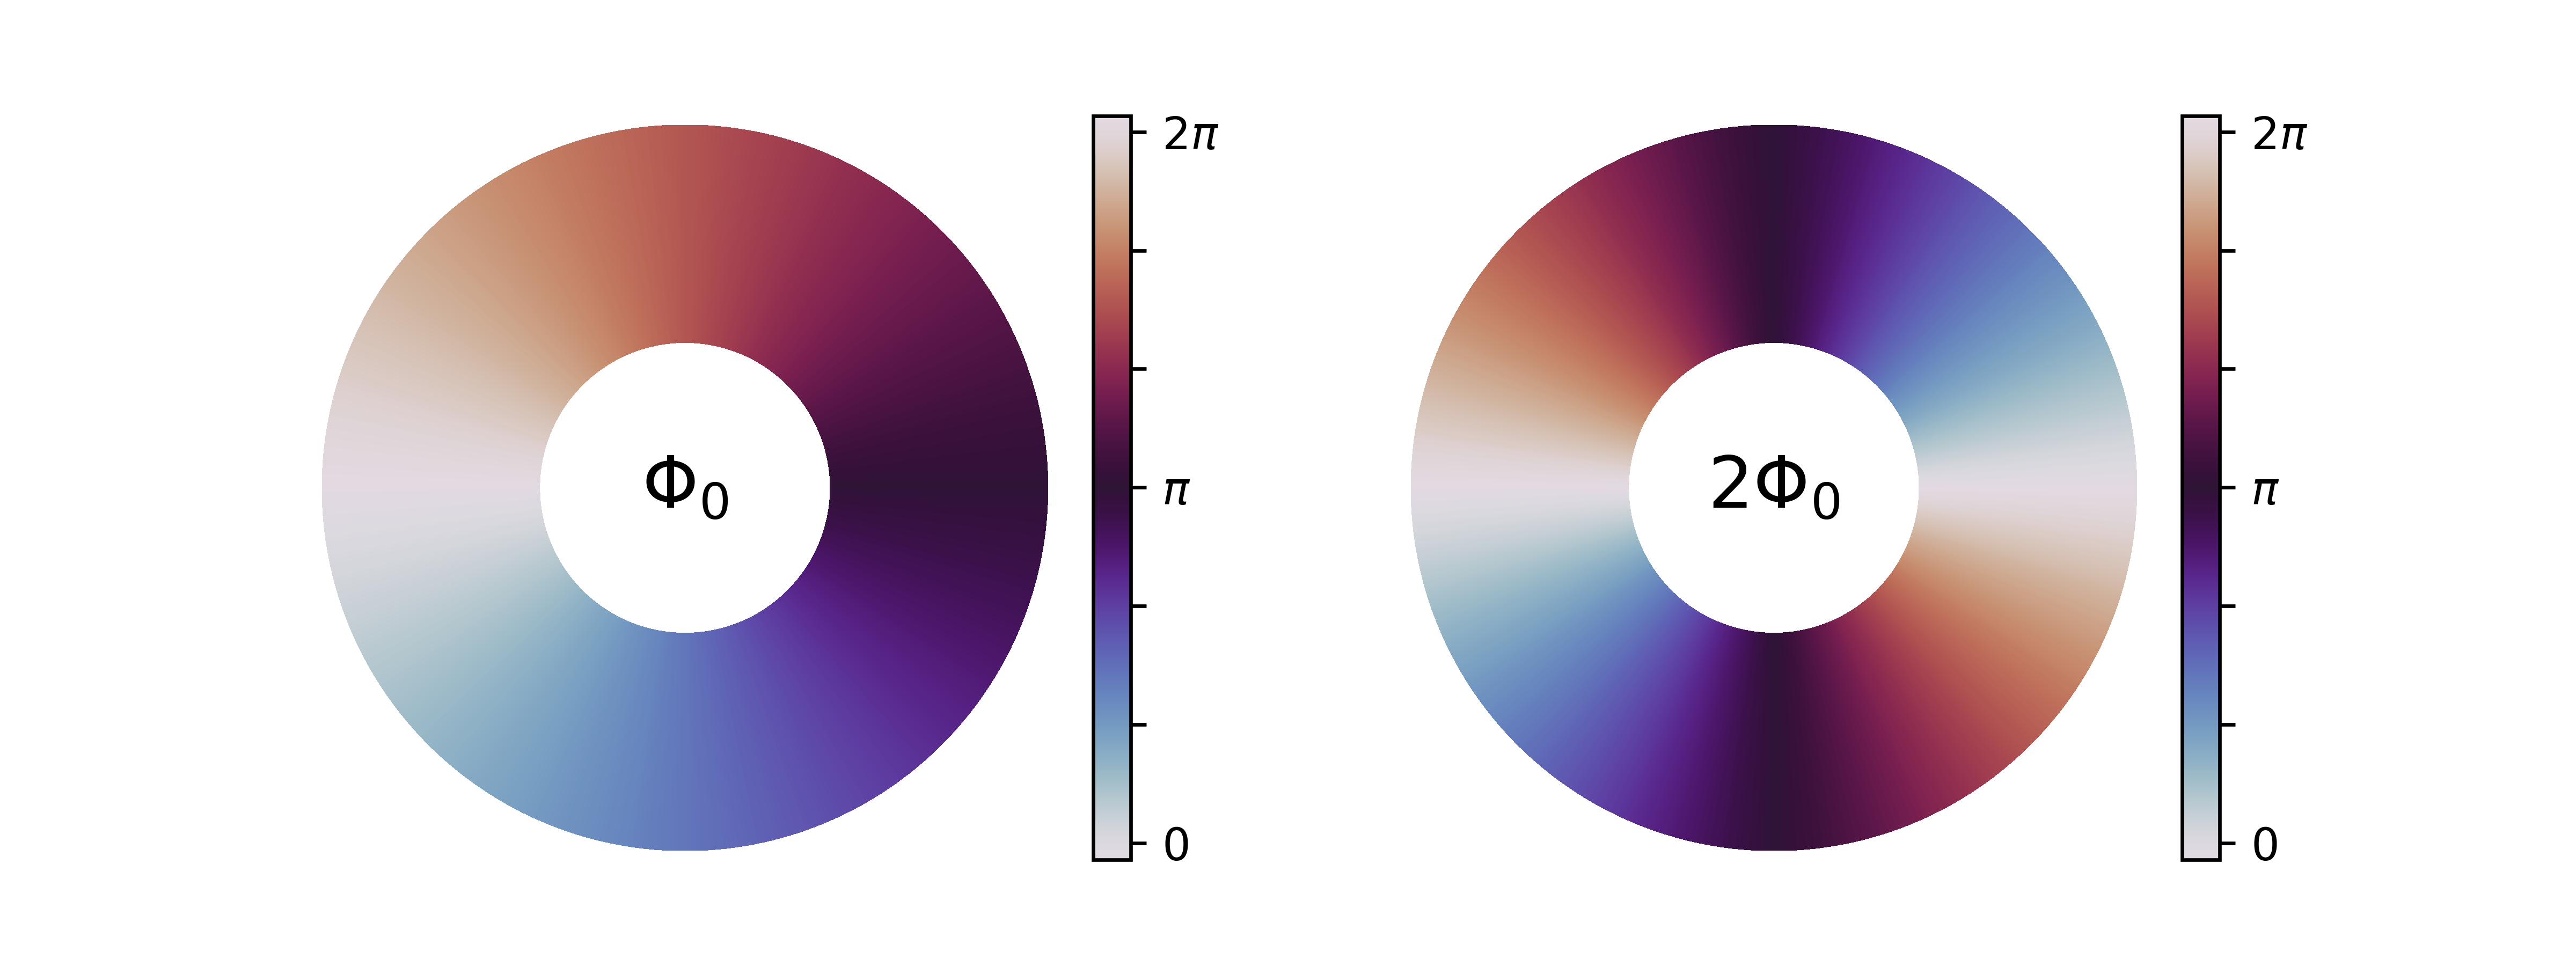
\includegraphics [width=1\textwidth] {coils}
	\caption{Распределение фазы волновой функции в сверхпроводящем кольце для различных значений магнитного потока.  }
	\label{img:coils}
\end{figure}
Квантование потока наглядно показывает, что во многих физических ситуациях, важных при описании сверхпроводниковых цепей, фаза оказывается очень тесно связанной с магнитным потоком. Экспериментально, квантование потока впервые наблюдалось в работе \cite{FluxQuant}.  Связь между $\varphi$ и $\Phi$ носит примерно такой же характер, как связь между $n$ и полным зарядом $Q$ сверхпроводящего острова. Действительно, у сверхпроводящего острова к дискретному заряду $Q_n \!=\! n\cdot2e$ добавляется заряд $q\! = \!CV$, наведённый некоторым напряжением $V$ через какую-либо дополнительную ёмкость $C$, и полный заряд равен $Q\!=\!Q_n\!+\!q$. Похожим образом, <<внутренний>> поток $LI_m$, возникающий за счет индуктивного ответа в кольце на внешнее магнитное поле, складывается с внешним потоком $\Phi_{ext}$, и в результате получается дискретный <<полный>> поток $\Phi\!=\!n\Phi_0$. Но как создать какую-либо наведенную непрерывным образом фазу? Оказывается, что при использовании эффекта Джозефсона это становится возможным.
\subsection{Эффект Джозефсона: общие принципы}
Чтобы понять суть эффекта Джозефсона, рассмотрим два объемных сверхпроводника (берега), разделенных слоем диэлектрика. Будем называть такую систему джозефсоновским переходом (или SIS-переходом). Если этот слой достаточно толстый, то берега никак не связаны между собой. Начнем мысленно уменьшать толщину диэлектрического слоя, и рано или поздно возникнет туннельный эффект. Туннелировать могут как отдельные электроны (квазичастицы), так и куперовские пары, существующие независимо для каждого берега. Но куперовские пары имеют удвоенную массу по сравнению с квазичастичными возбуждениями. Поскольку вероятность прохожения барьера экспоненциально падает с ростом массы частицы, то при какой-то толщине $h_1$ барьер станет прозрачным только для квазичастиц, не пропуская куперовские пары. Квазичастицы не формируют конденсат, поэтому такое одноэлектронное туннелирование принципиально не будет отличаться от сходных процессов в нормальных металлах или полупроводниковых структурах. Туннельный ток будет зависеть от плотности состояний, и поэтому будет отличен от нуля только при $V\!>\!2\Delta$, что впервые наблюдалось в работе \cite{GiaeverGap}. Хоть процесс туннелирования куперовских пар весьма маловероятен, но тем не менее, барьер уже достаточно прозрачен, и можно сказать, что волновая функция отдельных электронов из одного берега частично проникает в другой. Продолжим уменьшать толщину диэлектрика. Оказывается, что при некоторой толщине $h_2\!<\!h_1$ возникает когерентность во всей электронной системе. Можно сказать, что куперовские пары образуются из электронов, принадлежащих двум разным металлам одновременно. Эти пары увлекаются в один или другой металл, а направление и  скорость их увлечения зависит от разности сверхпроводящих фаз между берегами. То есть, ненулевой сверхпроводящий ток возникает при $V\!=\!0$. Описанные процессы туннелирования схематично изображены на Рис.\:\ref{img:jj_tunn}. Из качественного рассмотрения может показаться, что одночастичный ток и ток конденсата должны возникать при одинаковой толщине барьера, но в действительности джозефсоновский ток наблюдается при меньшем нормальном сопротивлении, чем одночастичный. Это связано с влиянием тепловых флуктуаций, которые растут с увеличением $R$. Детальное описание можно найти в \cite{Barone}. Покажем, как этот ток зависит от разности фаз.
\begin{figure}
{\centering 
\hfill
\fontsize{22pt}{22pt}\selectfont
\def\svgwidth{3.5in}%
\input{images/JJ_disser.pdf_tex}
\hfill
}
\caption{SIS переход и различные процессы туннелирования через барьер.}
\label{img:jj_tunn}
\end{figure}
\subsection{Токо-фазовое соотношение}

%Прежде чем перейти к описанию эффекта Джозефсона, рассмотрим упрощенную модель электронной системы в сверхпроводнике в представлении зонной структуры. Прежде всего, имеется конденсат куперовских пар, то есть все пары находятся на одном энергетическом уровне, который можно выбрать за нулевой: $E=0$. Если разорвать пару, то возникает 2 квазичастичных возбуждения (электрона) c энергией $E>\Delta$, и если электрон видит частично прозрачный барьер, то он может протунеллировать из сверхпроводника. Также возможен процесс, когда уже имеющийся электрон с другой стороны барьера Вопрос о плотности состояний квазичастиц в зависимости от энергии может быть рассмотрен в теории БКШ, которая дает ответ:


Будем считать, что каждый из берегов имеет собственные состояния конденсата куперовских пар в нем, которые можно описать при помощи макроскопической волновой функции: $\Psi_R\! =\! \sqrt{\rho_R}e^{i\varphi_R}$ и $\Psi_L \!=\! \sqrt{\rho_L}
e^{i\varphi_L}$, где $\rho_R, \rho_L$ --- плотности частиц. Состояние всего конденсата можно искать в виде $\Psi = \Psi_L\ket{L}\!+\!\Psi_R\ket{R}$, что означает, что общий конденсат куперовских пар когерентно распределится так, чтоб минимизировать энергию всей системы. В базисе состояний $\ket{R}, \ket{L}$ гамильтониан системы можно записать в виде:
\begin{equation}
H = E_L\cdot \ket{L}\bra{L} + E_R\cdot \ket{R}\bra{R} + T\cdot\big[ \ket{L} \bra{R}+\ket{R}\bra{L}\big],
\end{equation}
где последний член описывает туннелирование системы как целого и означает, что потенциальный барьер достаточно прозрачен, и некоторые пары из конденсата могут состоять из электронов находящихся по разные стороны от барьера. Теперь можно решить уравнение Шредингера $i\hbar d\Psi/dt\! =\! H\Psi$, распадающееся на два уравнения для амплитуд $\Psi_L$~и~$\Psi_R$: 
\begin{align}
	i\hbar \frac{d\Psi_R}{dt} & =E_R\Psi_R+T\Psi_L, \nonumber \\
    i\hbar \frac{d\Psi_L}{dt} & =E_L\Psi_L+T\Psi_R.
    \label{eq: je_deriv}
\end{align} 
Подставим выражения для $\Psi_L$~и~$\Psi_R$, и получим ответ для плотности сверхпроводящего (джозефсоновского) тока через барьер $J_s={d\rho_R}/{dt}=-{d\rho_L}/{dt}$:
\vspace{-1pt}
\begin{equation}
J=\frac{2T}{\hbar}\sqrt{\rho_R \rho_L}\sin \varphi = J_c \sin \varphi,
\label{eq: cur-phase}
\end{equation}
где $\varphi = \varphi_L-\varphi_R$. Если считать $\rho_L$ и $\rho_R$ константами, что будет справедливо, например, в случае подключения к внешнему источнику тока, то величина $J_c$, называемая плотностью критического тока, зависит только от свойств перехода, а именно от типа сверхпроводника и ширины туннельного барьера. Микроскопическая теория дает следующее выражение для критического тока $I_c$ джозефсоновского перехода в случае нулевой температуры и одинаковых сверхпроводников с $\Delta_L=\Delta_R=\Delta$:
\begin{equation}
I_c = \frac{\pi \Delta}{2eR_n},
\end{equation}
где $R_n$ --- остаточное сопротивление на переходе при $T \ge T_c$. Впервые стационарный эффект Джозефсона наблюдался в работе \cite{StatJosephsonExp}.
Зависимость $J=J(\varphi)$ вида \eqref{eq: cur-phase} характерна не только для туннельного SIS-перехода, но и для многих других типов слабой связи (например, мост Дайема, SNS- и SSeS-переходы \cite{LikharevWL, CPhiR_review}). 
\subsection{Фазо-потоковое соотношение}
Выше было рассмотрено квантование магнитного потока в сплошном кольце. Рассмотрим, как меняется ситуация при прерывании кольца некоторым количеством SIS-переходов ($n$ штук), плоскости которых перпендикуляры плоскости кольца, см. Рис.\:\ref{img:ph-fl}. Будем считать, что внешнее магнитное поле невелико, и можно не учитывать его проникновение в область диэлектрика (которое приводит к необычным эффектам в переходах, см., например, \cite{Schmidt}, \S\:24). Выберем замкнутый контур $C$, пролегающий в глубине кольца, и запишем уравнение \eqref{eq:2GL} с учетом обращающегося в ноль мейсснеровского тока:
\begin{equation}
\label{eq: FFR}
\oint\displaylimits_{C}^{} \mathbf{A} d\boldsymbol{\ell} = \frac{\Phi_0}{2\pi}\oint\displaylimits_{C}^{}\nabla\varphi d\boldsymbol{\ell}
\end{equation}
Правая часть этого выражения содержит интеграл от градиента фазы вдоль контура. Однако, фаза не является непрерывной функцией, а скачкообразно меняется на переходах. Поэтому в таком виде вычислять интеграл нельзя. Разобъем контур $C$ на несколько отрезков кривой $A_iB_i, i=1,\ldots n$, таким образом исключая короткие отрезки контура $C$, лежащие внутри переходов, из контура интегрирования. Будем считать что левый интеграл при этом не изменяется:
\begin{equation}\label{eq:int_cAdl}
\oint\displaylimits_{C}^{} \mathbf{A} d\boldsymbol{\ell} = \sum_{i=1}^{n}\int\displaylimits_{A_i}^{B_i} \mathbf{A} d\boldsymbol{\ell},
\end{equation}
поскольку ширины переходов достаточно малы, а векторный потенциал не имеет никаких особенностей в коротких отрезках контура $C$, лежащих внутри переходов, так как токи и магнитные поля нулевые. Теперь вычислим правый интеграл как:
\begin{equation}
\label{eq:int_phi}
\begin{alignedat}{2}
\oint\displaylimits_{C}^{}\nabla\varphi d\boldsymbol{\ell} = \sum_{i=1}^{n}\int\displaylimits_{A_i}^{B_i}\nabla\varphi d\boldsymbol{\ell} = \sum_{i=1}^{n}\varphi_{B_i}-\varphi_{A_i} & = \\ =\varphi_{A_1} + \sum_{i=1}^{n-1}(\varphi_{A_{i+1}}-\varphi_{B_i}) - \varphi_{B_n} & = 2\pi k + \sum_{i=1}^{n}(\varphi_{A_{i+1}}-\varphi_{B_i}) = \\ 
& =2\pi k + \sum_{i=1}^{n}\delta\varphi_i,
\end{alignedat}
\end{equation}
В предпоследнем равенстве использовано условие однозначности волновой функции в виде $\varphi_{A_1} = \varphi_{A_{n+1}}-2\pi k$. Разности фаз на переходах обозначены как $\delta\varphi_i$. Подставляя \eqref{eq:int_cAdl} и \eqref{eq:int_phi} в \eqref{eq: FFR}, получаем искомое фазо-потоковое соотношение:
\begin{equation}
\label{eq: FFR_final}
\frac{2\pi\Phi}{\Phi_0} = 2\pi k + \sum_{i=1}^{n}\delta\varphi_i.
\end{equation}
Таким образом, поток в таком кольце не квантуется, но однозначно определяется разностями фаз на джозефсоновских переходах. Предположим, например, что джозефсоновские энергии переходов, входящих в кольцо, одинаковы и равны $E_J$, соответственно, равны и критические токи $I_c$. Тогда
\begin{equation}\label{eq: FFR_case}
\frac{2\pi}{\Phi_0}(\Phi_{ext}-LI_c\sin \delta\varphi)= 2\pi k + n\delta\varphi,
\end{equation}
и при заданных $L\text{ и }\Phi_{ext}$ можно найти такие $k \text{ и } \delta\varphi$, которые характеризуют разрешенные состояния системы. Если переходы различны, то разности фаз $\delta\varphi_i$ будут такими, чтобы токи через переходы $I_i=I_{ic}\sin\delta\varphi_i$ были одинаковыми. 
\begin{figure}
	\centering
		\fontsize{22pt}{22pt}\selectfont
		\def\svgwidth{3.5in}%
		\input{images/phase-flux2.pdf_tex}
	\caption{К выводу фазо-потокового соотношения.}
	\label{img:ph-fl}
\end{figure}
%\begin{figure}[ht] 
%	\centering
%	\includegraphics [width=1\textwidth] {coils_jj.png}
%	\caption{Распределение фазы волновой функции в сверхпроводящем кольце для различных значений магнитного потока.}
%	\label{img:coils_JJ}
%\end{figure}
\subsection{Энергия джозефсоновского тока. RSCJ-модель.}
Из уравнений \eqref{eq: je_deriv} можно получить следующее соотношение:
\begin{equation}
\frac{d\varphi}{dt} = \frac{2eV}{\hbar}.
\label{eq: dphidt}
\end{equation}
Таким образом, при конечном напряжении на контакте фаза начинает меняться с течением времени. Это так называемый нестационарный эффект Джохефсона, имеющий множество интересных применений, например генерация высокочастотного тока и создание стандарта напряжения. Используя полученное соотношение, можно рассчитать потенциальную (свободную) энергию, сосредоточенную в переходе:
\begin{equation}
\label{eq:EJ}  
E(\varphi) = \int_{0}^{t}I_sVdt = \int_{0}^{\varphi} I_c\sin \varphi' \frac{\hbar}{2e} {d\varphi'} = E_J(1-\cos\varphi).
\end{equation}
В последнем равенстве учтено что при нулевой фазе ток через переход не течет, и $E(0)=0$. Величина $E_J = {\hbar I_c}/{2e}$ называется \textit{джозефсоновской энергией} перехода. При малых значениях $\varphi$ энергия квадратично зависит от фазы: $E_J\approx E_J \varphi^2/2$, что дает возможность ввести эквивалентную линейную индуктивность перехода $L_{lin} = \Phi_0^2/2\pi I_c$. В более общем случае, джозефсоновская индуктивность зависит от фазы и определяется как $L_J = \Phi_0/(2\pi I_c \cos \varphi)$.
\begin{figure}[ht]
	{\centering
		\hfill
%		\subbottom[List-of-Figures entry][Туннельные процессы в SIS-переходе.\label{img:jj_tunnel}]{%
%			\input{images/JJ_disser.pdf_tex}}
%		\hfill
		\subbottom[List-of-Figures entry][RCSJ-модель перехода.]{%
			\input{images/RSCJ.pdf_tex}}
		\label{img:RCSJ}
		\hfill
		\def\svgwidth{2.2in}
		\subbottom[Частица в потенциале $U(\varphi)$.]{%
			\input{images/washboard.pdf_tex}}
		\label{fig: washboard}
		\hfill
	}
	\caption{RCSJ-модель джозефсоновского туннельного перехода.}
	\label{img:knuth_2}
\end{figure}

До сих пор мы рассматривали лишь энергию сверхпроводящего тока. Однако, для описания нестационарных процессов в реальных туннельных контактах такая модель недостаточна. Необходимо учитывать два дополнительных фактора: квазичастичное туннелирование и значительная емкость между двумя сверхпроводниками, неизбежно возникающая из-за малой толщины диэлектричекой прослойки (несколько десятков межатомных расстояний). Эти аспекты учитываются в феноменологической RCSJ-модели перехода, в которой параллельно с джозефсоновским элементом, энергия которого зависит от фазы согласно \eqref{eq:EJ}, включается эквивалентный резистор $R$, описывающий нормальное сопротивление квазичастичному току, и конденсатор $C$, см.\:Рис.\:\ref{img:RCSJ}. Полный ток через переход в такой схеме можно записать как:
\begin{align}
I &= I_C + I_J + I_R = \frac{\hbar C}{2e} \frac{d^2\varphi}{dt^2}+I_c\sin \varphi+ \frac{\hbar}{2eR}\frac{d\varphi}{dt}, \text{ отсюда получаем:}  \nonumber \\
0 & = m\frac{d^2\varphi}{dt^2} + f \frac{d\varphi}{dt} + \frac{d}{d\varphi}\big(E_J\cos \varphi+E_J\frac{ I}{I_c}\varphi\big), 
\end{align}
где введены обозначения $m=(\hbar/2e)^2 C$ и $f=(\hbar/2e)^2R^{-1}$. Полученное уравнение описывает динамику фазы в переходе как классическое движение частицы массой $m$ в жидкой среде с коэффициентом вязкости $f$ во внешнем потенциале стиральной доски $U(\varphi)=-E_J(\cos \varphi+I\varphi/I_c)$, что схематично отражено на Рис.\:\ref{fig: washboard}. Отметим некоторые характерные особенности динамики системы:
\begin{itemize}
	\item При отсутствии тока потенциал синусоидален, и частица локализуется в потенциальной яме, форма которой близка к параболической, и в этом случае может совершать малые колебания с частотой $\omega_p = (\sqrt{L_{lin}C})^{-1}$, называемой \textit{плазменной частотой перехода}. 
	\item Если увеличивать ток, то наклон потенциала растёт, потенциальная яма становится все более мелкой и пропадает. Частица начинает двигаться и будет разгоняться вдоль стиральной доски, пока не достигнет режима, в котором среднее значение $\langle V \rangle  \propto \langle d\varphi/dt \rangle$ постоянно и отлично от нуля. Характер её замедления при уменьшении тока (наклона) определяется параметром Маккамбера $\beta_c = \omega_p R C$, который показывает обратное число плазменных колебаний, которые система может совершить за время затухания $RC$ (при отсутствии тока).
	\item Если $\beta_c\ll1$, то при уменьшении тока частица практически не замедляется до тех пор, пока наклон не упадет практически до нуля. 
	\item Если $\beta_c\gg1$, то частица замедляется довольно значительно, так как трение играет существенную роль в её движении и скорость движения вдоль стиральной доски определяется средним наклоном. Полная остановка, однако, также произойдет лишь при $I=0$.
\end{itemize}
Перечисленные особенности находят подтверждение при измерении ВАХ переходов, полученных при фиксированном внешнем токе $I$, см., например, \cite{Schmidt}. 

Подведем итог классическому описанию джозефсоновского перехода. В зависимости от выбранного режима работы, такой переход может вести себя как нелинейный осциллятор, нелинейная индуктивность, зависящая от времени, либо демонстрировать еще более сложное поведение. Это делает его весьма интересным элементом даже с точки зрения классической схемотехники. Еще более нетривиальные эффекты возникают в том случае, если рассматривать разность фаз на переходе как квантовую степень свободы, которые мы кратко опишем далее. 
\section{Квантование электрических цепей}
\label{ch: Quant}

Как было сказано выше, при квантовом описании какой-либо сверхпроводящей системы число пар $\hat{n}$ на сверхпроводящем острове и фаза $\hat{\varphi}$ на этом острове могут рассматриваться как сопряженные переменные: $[\hat{\varphi}, \hat{n}]=i$. Возбуждения коллективной квантовой степени свободы при определенных условия оказываются самыми низкоэнергетическими (ниже 10 ГГц), и потому есть возможность экспериментально работать только с ними. В сверхпроводниках минимальная энергия одноэлектронного возбуждения не может быть меньше $2\Delta$, например, для алюминия имеем $2\Delta=3.52 k_b T_c\approx h\cdot80$ ГГц. Можно показать \cite{girvin2011circuit}, что частоты объемных плазменных колебаний попадают в терагерцовый диапазон, и поэтому их также можно исключить из рассмотрения. Фактически, мы будем иметь дело с бездисперсионными коллективными плазменными возбуждениями, и именно эти моды в итоге будут квантоваться. 
\subsection{Кубит. Двухуровневое приближение. Приближение вращающейся волны.}
\label{sec: qubit}
Простейшая квантовая система, например, спин $1/2$ в продольном магнитном поле, обладает одной степенью свободы и двумя собственными квантовыми состояниями. Обозначим состояния системы как $\ket{0}\equiv\begin{pmatrix} 1 & 0 \end{pmatrix}^{T} \text{и} \ket{1}\equiv\begin{pmatrix} 0&1 \end{pmatrix}^T$, а соответствующие собственные значения энергии как -$E_q/2$ и $E_q/2$. Тогда гамильтониан кубита записывается тривиально: $\hat{H}\!=\!\frac{-E_q}{2}\sz$. 

Согласно постулату квантовой механики, все возможные состояния кубита записываются как~$\ket{\psi}=\cos\frac{\theta}{2}\ket{0}+ 
e^{i\varphi}\sin\frac{\theta}{2}\ket{1}, 0 \le \theta \le \pi, 0 \le \varphi \le 2\pi $. Любая реальная система взаимодействует со своим окружением, поэтому состояния кубита необходимо описывать матрицей плотности:
\begin{equation}
\rho_q = \ket{\psi}\bra{\psi} =
\begin{pmatrix} \cos^2\frac{\theta}{2} & \cos\frac{\theta}{2}e^{-i\varphi}\sin\frac{\theta}{2}\\
\cos\frac{\theta}{2}e^{i\varphi}\sin\frac{\theta}{2}& \sin^2\frac{\theta}{2}
\end{pmatrix} = 
\begin{pmatrix} 1-\rho_{11} & \rho_{01}\\ \rho_{01}^*& \rho_{11}
\end{pmatrix}
\end{equation}
Последнее выражение можно обобщить и на случай смешанных состояний кубита, которые описывают статистический ансамбль. Поскольку матрицы Паули вместе с единичной матрицей составляют базис в пространстве матриц $2\times2$, то такую матрицу плотности можно записать в общем виде:
\begin{equation}
\rho_q = \frac{1}{2}(I+\vec{s}\cdot\vec{\sigma}),
\label{eq: rho_to_bloch}
\end{equation}
где $I$ --- единичная матрица, $\vec{\sigma}=\begin{pmatrix} \sigma_x & \sigma_y & \sigma_z \end{pmatrix}^{T}$ и
 $\vec{s}=\begin{pmatrix} s_x & s_y & s_z \end{pmatrix}^{T}$ --- трёхмерный вектор, называемый вектором Блоха. Для чистых состояний $\vec{s}=\begin{pmatrix} \sin\theta\cos\varphi & \sin\theta\sin\varphi & \cos\theta \end{pmatrix}^{T}$ можно представить как вектор из начала координат единичной длины, и все возможные положения конца этого вектора формируют единичную сферу --- сферу Блоха, см. Рис. \ref{img:bloch}.
\begin{figure}
 	\centering
 	\def\svgwidth{4in}
 	\input{images/Bloch_empty_3.pdf_tex}
 	\caption{Сфера Блоха. Точки на сфере соответствуют чистым состояниям кубита, точки внутри сферы --- смешанным состояниям.}
 	\label{img:bloch}
\end{figure} 

Квантовая двухуровневая система является простейшим объектом. В реальных экспериментах с СКЦ мы, как правило, работаем с многоуровневой системой. Но в некоторых физических ситуациях можно выделить два нижних уровня системы, и рассматривать систему внутри подпространства из основного и первого возбужденного квантовых состояний. 
Для этого необходимо делать двухуровневое приближение. 

Рассмотрим систему с собственными состояниями $\hat{H}_0\ket{n} = E_n\ket{n}$, под действием возмущения $\hat{V}(t)$. Учитывая поправку к собственным энергиям ${\tilde{E}_n}=E_n+\braket{n|\hat{V}|n}$, можно записать полный гамильтониан в виде:
\begin{equation}
\hat{H} = \sum_n\tilde{E}_n\ket{n}\bra{n} + \sum_{m \ne n}\textbf{}\ket{m}\bra{n}\braket{m|\hat{V}|n}. 
\end{equation} 
Оператор эволюции можно записать через повышающие и понижающие матрицы: $\hat{V} =   \sum_{m>n}\braket{m|\hat{V}|n}\hat{\sigma}_{mn}+\braket{n|\hat{V}|m}\hat{\sigma}_{nm}$. Тогда оператор эволюции возмущенной системы $U_0(t) = \exp(-\frac{i}{\hbar}(\tilde{E}_n\ket{n}\bra{n}))$ задаёт представление взаимодействия, гамильтониан в котором имеет вид:
\begin{equation}\label{eq: H_I}
\hat{H}_I = \sum_{m>n} e^{-{i}(\tilde{\omega}_n-\tilde{\omega}_m)t}\braket{m|\hat{V}|n}\hat{\sigma}_{mn} + \text{ c.c} 
\end{equation}
Если возмущение будет состоять из нескольких слагаемых, то соответствующие $\hat{H}_I$ могут не коммутировать, что сильно усложнит поиск аналитического решения для динамики системы и приведет к непоправимым последствиям. Однако, предположим, что $\hat{V}(t)\!=\!\hat{V}_0e^{i\omega t}$, где $\omega\!\approx\!\tilde{\omega}_{01}$. Тогда ясно, что наибольший вклад в оператор эволюции системы в представлении взаимодействия $\mathcal{T} \exp (-\frac{i}{\hbar}\int_0^t \hat{H}_I(t')dt')$ даёт слагаемое из \eqref{eq: H_I} с наиболее медленной зависимостью от времени. Все остальные члены дают интегралы от быстро осциллирующих функций, которые очень малы и не меняют характер динамики, заданной главным членом. Таким образом, мы можем сделать два приближения:
\begin{itemize}
	\item \textit{двухуровневое приближение} позволяет оставить в $H_I$ только члены $\braket{0|\hat{V}_0|1}\hat{\sigma}_{01} + e^{-2\omega t}\braket{1|\hat{V}_0|0}\hat{\sigma}_{10}$, пренебрегая переходами между остальными парами уровней, не попадающими в резонанс с возмущающим воздействием;
	\item \textit{приближение вращающейся волны} позволяет оставить только медленно меняющийся член $\braket{0|\hat{V}_0|1}\hat{\sigma}_{01}$.
\end{itemize}

Для того чтоб описывать СКЦ как кубит, необходимо, во-первых, уметь рассчитать её спектр в зависимости от параметров цепи и, во-вторых, уметь вычислить матричные элементы переходов под воздействием возмущений, например, внешнего электромагнитного поля. Теперь опишем общий формализм квантования цепи, а затем на некоторых примерах покажем, как осуществляются расчеты такого типа.
\subsection{Формальная процедура квантования цепи}	
Опишем общий подход к квантованию СКЦ \cite{vool2017introduction}. Будем рассматривать некоторую систему, состоящую из набора сверхпроводящих островов. Острова могут быть связаны взаимными емкостями и индуктивностями. Кроме того, некоторые из них могут образовывать джозефсоновскую связь. Поэтому, достаточно общим является представление такой системы в качестве электрической цепи, в которой имеются три типа элементов: емкости, индуктивности и джозефсоновские элементы (нелинейные индуктивности)\footnote[1]{Совсем недавно \cite{astafiev2012coherent} показана возможность создания т.н. центра когерентного квантового проскальзывания фазы, который является емкостным аналогом джозефсоновского перехода. Однако, создание квантовых цепей из таких элементов еще не вполне отработано. Их описание выходит за рамки данной работы.}. Как и в электротехнической цепи, в такой системе нужно подходящим образом выбрать некоторые независимые степени свободы, с помощью которых можно описать как классическую, так и квантовую динамику системы. Последовательность действий квантования системы состоит из следующих шагов:
\begin{enumerate}
\item Изобразим эквивалентную электрическую схему цепи. Схема будет состоять из N узлов (точек), связанных произвольным количеством элементов-двуполюсников, которые мы будем называть ребрами. Мысленно выделим емкостную и индуктивную части в общей схеме цепи. Поскольку любой реальный элемент имеет конечные размеры, и следовательно, паразитную емкость, то можно считать, что между каждой парой узлов включена емкость, и притом единственная. Среди всех узлов можно выделить \textit{активные} узлы, к которым подсоединены как емкостные, так и индуктивные элементы, и \textit{пассивные} узлы, к которым подсоединены только емкости.

\item Для каждого ребра введем величину $\Phi(t)=\int_{-\infty}^{t} v(t')dt'$, которую можно назвать магнитным потоком через ребро. Считается, что напряжение $v(-\infty)=0$ и плавно включается со временем. Тогда емкостную энергию можно записать как $C\dot{\Phi}^2/2$, что соответствует кинетической энергии частицы с кординатой $\Phi$. Для индуктивности эта величина в точности совпадает с запасённым в ней магнитным потоком, и индуктивная энергия $(\Phi-\widetilde{\Phi})^2/2L$ играет роль потенциальной энергии, где $\widetilde{\Phi}$ --- некоторый внешний поток. 
\item Выберем один из активных узлов емкостной подсистемы в качестве заземленного узла, и выберем только те емкости, которые единственным образом соединяют земляной узел со всеми остальными узлами подсистемы. Эти емкости составят \textit{остовное дерево} $T$. Тогда для любого другого узла $n$ можно ввести т.н. \textit{узловой поток} $\phi_n$, который равен сумме потоков всех емкостей, через которые нужно пройти от земляного узла до узла $n$. Связь между потоком через некоторое ребро $\Phi_b$ и потоками через узлы этого ребра $\phi_n, \phi_{n'}$ даётся соотношением:
\begin{equation}\label{eq: Phiphi}
\begin{aligned}
	\Phi_{b\in T} &= \phi_n-\phi_{n'}, \\
	\Phi_{b\notin T} &= \phi_n-\phi_{n'} + \widetilde{\Phi}_b,
\end{aligned}
\end{equation}
где внешний поток ${\Phi}_b$ учитывается в том случае, когда добавление ветви $b$ образует индуктивную петлю.
\item Используя соотношения \eqref{eq: Phiphi}, запишем полную энергию индуктивной и емкостной подсистемы через переменные $\vec{\phi}=(\phi_1\ldots\phi_N)^T$.  Энергия индуктивной подсистемы примет вид:
\begin{equation}
E_L(\vec{\phi}) = \frac{1}{2}{\vec{\phi}^{\mathsmaller T}} \mathbf{L^{-1}}\vec{\phi} + \sum_b \frac{\phi_n-\phi_{n'}}{L_b}\widetilde{\Phi}_b.
\end{equation}
Первое слагаемое представляет собой вклад в энергию непосредственно от индуктивностей. Матрица индуктивности $\mathbf{L}$ размера $(N-1)\!\times\!(N-1)$ симметричная и сконструирована следующим образом: недиагональные элементы $(i,j)$ равны $-\sum L_{ij}$, где $L_{ij}$ - все индуктивности, соединяющие узлы $i$ и $j$; диагональные же элементы равны сумме всех недиагональных элементов на соответствующей строке (или в столбце), взятой с противоположным знаком. Второе слагаемое --- это энергия каждой индуктивности, которая находится в ветви с внешним потоком $\widetilde{\Phi}_b$. Энергия емкостной подсистемы примет вид:
\begin{equation}
E_C(\dot{\vec{\phi}})= \frac{1}{2} {\dot{\vec{\phi}}^{\mathsmaller T}} \mathbf{C^{-1}} \dot{\vec{\phi}}
\end{equation}
где матрица емкости $\mathbf{C}$ строится аналогично матрице индуктивности.
\item Полученные выражения позволяют записать лагранжиан системы $\mathcal{L} = E_C-E_L$ и найти классические уравнения движения $\frac{d}{dt}\frac{\partial\mathcal{L}}{\partial\dot{\phi_n}}=\frac{\partial\mathcal{L}}{\partial{\phi_n}}$. Поскольку нас интересует квантовое описание системы, необходимо найти обобщенные импульсы $q_n = \partial\mathcal{L}/\partial{\dot\phi_n}$,  и записать гамильтониан $H = q_n\phi_n-\mathcal{L}$. Сколько независимых степеней свободы будет иметь система? Чтобы ответить на этот вопрос, необходимо заметить, что для любого пассивного узла $\partial \mathcal{L}/\partial{\phi_n}=0$, а поэтому $q_n$ является константой, и фактически, даннная степень свободы вырождена. Таким образом, если число активных узлов $P$, то полное число степеней свободы $P-1$.
\item Заменяя координаты (узловые потоки) и импульсы (узловые заряды) на сопряженные операторы $\phi\rightarrow\hat{\phi}$~и~$q\rightarrow\hat{q} = -i\hbar\frac{\partial}{\partial \phi}$, получаем гамильтониан квантовой цепи. Далее можно найти стационарные состояния, их энергии, матричные элементы переходов, и описать динамику системы.
\end{enumerate}
Далее мы рассмотрим некоторые базовые типы СКЦ. Как правило, они достаточно просты, и можно записать гамильтониан практически сразу, без предварительных шагов. Однако, следование общему формализму квантования необходимо для правильного описания более сложных цепей со многими степенями свободы. 
   
Базовые типы СКЦ, далее просто кубитов - это зарядовый кубит, фазовый кубит, потоковый кубит, трансмон и вч-СКВИД. Кратко опишем свойства каждого из этих кубитов.
\subsection{Зарядовый кубит}\label{charge_q}
	\begin{figure}[b]
		{ \raggedleft
			\hfill
			\def\svgwidth{2in}
			\fontsize{19pt}{19pt}\selectfont
			\subbottom[List-of-Figures entry][\label{img: CPB_scheme}]{%
				\input{images/CPB_qubit.pdf_tex}}
			\hfill
			\def\svgwidth{4in}
			\subbottom[\label{img: CPB_spectrum}]{%
				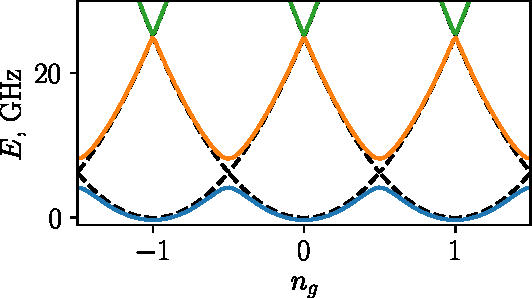
\includegraphics{images/CPB_spectrum.pdf}}
			
			\hfill
		}
		\caption[Схема зарядового кубита и его спектр.]{Зарядовый кубит: a) Эквивалентная схема кубита, б) Спектр кубита: три нижних энергетических уровня в зависимости от $n_g$. $E_C/h=\!=\!50 \text{ ГГц}, E_J/h\!=\!4\text{ ГГц}$. Пунктирная линия показывает классическую зарядовую энергию в отсутствие туннелирования.}
		\label{img: CPB}
		
	\end{figure}
Зарядовый кубит, или <<ящик>> для куперовских пар - это система, представляющая из себя джозефсоновский переход с энергией $E_J$, последовательно соединённый с емкостью. Эквивалентная схема такого кубита изображена на Рис.\ref{img: CPB}\subcaptionref*{img: CPB_scheme}. Образуется изолированный остров (выделен синим цветом), и если его емкость достаточно мала, то изменение числа куперовских пар на единицу сильно меняет энергию системы.  Введем зарядовую энергию конденсатора $E_C = 4e^2/C$; она включает в себя всю эффективную емкость острова, в т.ч. джозефсоновскую емкость. Также к острову подключен внешний источник, который может создавать наведенный заряд $n_g = C_gV_g/2e$.   Остовное дерево и земля выбираются тривиально, и понятно, что единственная степень свободы задается операторами фазы $\hat{\varphi}_1\!=\!2\pi/\Phi_0\!\cdot\!\hat{\phi}_1$ и заряда $\hat{n}_1\!=\!\hat{q}_1/2e$, далее индекс будет опущен за ненадобностью.~Гамильтониан системы имеет вид:
\begin{equation}
\hat{H}_{CPB} = \frac{E_C}{2}(\hat{n}-n_g)^2-E_J \cos \hat{\varphi}.
\end{equation}
Для нахождения спектра можно выбрать как фазовый базис, в котором $\hat{\varphi}\!=\!\varphi$, так и базис чисел куперовских пар (зарядовый базис), в котором $\hat{n}\!=\!n$. Начнем рассмотрение с зарядового базиса и выясним, как записать оператор $\cos\hat{\varphi}$. Заметим, что:
\begin{equation}
e^{i\hat{\varphi}}\ket{n} = e^{i\hat{\varphi}}\sum_n e^{in\hat{\varphi}}\ket{\varphi} = \ket{n+1},
\end{equation}
поэтому имеем:
\begin{equation}\label{eq: cosphi}
\cos \hat{\varphi} = \frac{1}{2}(e^{i\hat{\varphi}}+e^{-i\hat{\varphi}}) =
\frac{1}{2}\sum_n\Big(\ket{n+1}\bra{n} + \ket{n}\bra{n+1}\Big),
\end{equation}
где во втором слагаемом последнего выражения был сдвинут индекс суммирования $n \rightarrow n+1$. Гамильтониан можно записать в виде:
\begin{equation}
\hat{H}_{CPB} = \frac{E_C}{2}\sum_n(n-n_g)^2\ket{n}\bra{n}-\frac{E_J}{2} \sum_n\Big(\ket{n+1}\bra{n} + \ket{n}\bra{n+1}\Big).
\end{equation}
Получив его в такой форме --- диагональная часть плюс туннельный гамильтониан --- можно сразу сказать, как будет выглядеть собственные уровни энергии: в случае полуцелых $n_g$ два состояния с соседними $n$, вырождены. Новые собственные состояния сдвинуты на $\pm E_J/2$. Численно рассчитанный спектр изображен на Рис. \ref{img: CPB}\subcaptionref*{img: CPB_spectrum}. Сделаем двухуровневое приближение, то есть будем рассматривать подсистему из двух зарядовых состояний $\ket{0}$ и $\ket{1}$, и считать, что $n_g \approx 0.5$. Тогда гамильтониан примет вид: 
\begin{equation}
H_q = \frac{E_C}{2}(n_g-1/2)\sz-\frac{E_J}{2}\sx, 
\end{equation}
а новые собственные состояния системы можно записать через параметр $\theta = \arctan(\frac{2E_J}{E_C(n_g-1/2)})$ следующим образом: 
\begin{equation}
\begin{aligned}
\ket{g} & = \sin \frac{\theta}{2} \ket{0} + \cos \frac{\theta}{2} \ket{1}, \\
\ket{e} & = \cos \frac{\theta}{2} \ket{0} - \sin \frac{\theta}{2} \ket{1}
\label{eq: charge_e}
\end{aligned}
\end{equation}
Как и следовало ожидать, состояния максимально гибридизованы в окрестности $n_g\!=\!1/2$. 

Считается, что в пределе зарядового кубита $E_J < E_C$, то есть туннеллирование проявляется лишь между соседними зарядовыми состояниями. Отчасти исследование именно такого режима связано с тем, что зарядовый кубит --- исторически первый кубит, который был продемонстрирован в эксперименте \cite{nakamura1999coherent}. Для считывания используются такие методы, как джозефсоновский цикл квазичастичной генерации через дополнительный пробный барьер, подключенный к острову, а также одноэлектронный транзистор \cite{pashkin2009josephson}. Для такого считывания требуется, чтоб энергии зарядовых состояний при фиксированном $n_g$ сильно отличались друг от друга, то есть, ярко выраженный эффект кулоновской блокады. С этим связан и существенный недостаток зарядового кубита --- слишком высокая чувствительность к зарядовому шуму, влияющему на $n_g$. Различные паразитные двухуровневые системы в кремниевой подложке обладают электрическим дипольным моментом, влияющим на энергию кубита. Кроме того, попадание любой случайной квазичастицы на остров сильно сдвигает рабочую точку и делает длительную когерентную манипуляцию невозможной. В дальнейшем мы рассмотрим модификацию зарядового кубита с малой зарядовой энергией --- кубит-трансмон, работающий в так называемом пределе плоских зон, когда чувствительность к зарядовым шумам практически исчезает.
\subsection{Фазовый кубит}
Еще один тип кубитов, активно использовавшийся в 2000-х гг. --- фазовые кубиты \cite{martinis2009superconducting}. Фазовый кубит представляет собой смещенный постоянным током джозефсоновский переход. Точный контроль значения тока смещения $I$ позволяет хорошо контролировать глубину ямы в потенциале стиральной доски, см.~Рис. \ref{fig: washboard} и таким образом, регулировать число квантовых состояний, локализованных в яме. Пара нижних уровней и используется в качестве кубитной подсистемы. Управление осуществляется внешним высокочастотным током, подаваемым на переход. Считывание состояний \cite{steffen2006measurement} осуществляется при помощи дополнительной потоковой линии контроля: короткий импульс постоянного тока дополнительно наклоняет потенциал стиральной доски. Величина этого наклона подобрана таким образом, чтобы переход в состоянии $\ket{1}$ имел очень высокую вероятность протуннелировать через потенциальный барьер, который на время импульса становится значительно более прозрачным. В то же время, вероятность туннелирования состояния $\ket{0}$ должна быть исчезающе мала. Этого не так сложно добиться, учитывая тот факт, что согласно квантовой механике, в любой сколь угодно мелкой одномерной потенциальной яме имеется связанное состояние. Если туннелирование произошло, то джозефсоновский переход начинает движение вдоль стиральной доски, и на нём появляется ненулевое напряжение, и как следствие, высокочастотная компонента тока. Её можно обнаружить при помощи дополнительного считывающего СКВИДa, что и делается в эксперименте. Как легко заметить, такое считывание разрушает кубит, и требуется конечное время для последующей инициализации в состоянии $\ket{0}$. Кроме того, шум тока смещения может вызывать значительное изменение потенциала, и как следствие, дефазировку кубита. Несмотря на имеющиеся недостатки, в работе с данными кубитами достигнут серьезный прогресс: были созданы 4-кубитные квантовые процессоры \cite{lucero2012computing}, реализующие простейшие квантовые алгоритмы, например, разложение на множители числа 15. В настоящий момент интерес к данному типу кубитов несколько уменьшился, однако, их исследование в достаточной мере способствовало развитию физики СКЦ.
 
\subsection{Потоковый кубит}
\label{subsec: flux_q}
В зарядовом кубите, который мы рассмотрели ранее, реализуется суперпозиция состояний с разными числами куперовских пар на острове. Похожим образом можно создать суперпозицию состояний с различным значением магнитного потока в сверхпроводящей петле с включенными в неё джозефсоновскими переходами. Данная концепция была предложена в работе \cite{mooij1999josephson}, а кубит получил название <<кубит с незатухающим током>> и впоследствии упоминался упрощенно как \textit{потоковый кубит}. Схема потокового кубита с тремя джозефсоновскими переходами приведена на Рис.~\ref{img: flux_q}\subcaptionref*{img: fluxQ_scheme}. Обычно два перехода одинаковые, а площадь третьего перехода составляет $\alpha$ от площади больших переходов. Обычно выбирается $0\!<\!\alpha\!<\!1$. 
\begin{figure}[b]
	{ \raggedleft
		\hfill
		\def\svgwidth{3in}
		\fontsize{19pt}{19pt}\selectfont
		\subbottom[List-of-Figures entry][\label{img: fluxQ_scheme}]{%
			\input{images/3jj_qubit_ed.pdf_tex}}
		\hfill
		\subbottom[\label{img: flux_spectrum}]{%
			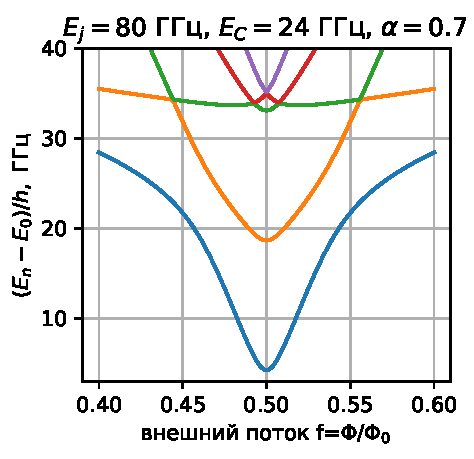
\includegraphics[width=0.5\textwidth]{images/3jj_spectrum_2.pdf}}
		
		\hfill
	}
	\caption[Схема потокового кубита и его потенциальная энергия.]{Потоковый кубит: a) Эквивалентная схема кубита, б) Спектр кубита: зависимости низших энергетических уровней в зависимости от $\Phi/\Phi_0$.}
	\label{img: flux_q}
	
\end{figure}

Запишем лагранжиан системы, используя операторы потока в узлах $\phi_i, i=\{1,2\}$ и их фазовые аналоги $\varphi_i=2\pi\phi_i/\Phi_0$:
\begin{multline}\label{eq: Lagr_flux}
{\mathcal{L}} = \frac{C}{2}
\begin{pmatrix}\dot{\phi}_1 &\dot{\phi}_2\\
	\end{pmatrix}
\begin{pmatrix}
	2 & -1\\ 
	-1 & \alpha+1 \\
\end{pmatrix}
\begin{pmatrix}\dot{\phi}_1\\\dot{\phi}_2\\\end{pmatrix}
%\Big[\frac{{\dot{\phi}}^2_1}{2}+ \frac{({ {\dot{\phi}}_2-{\dot{\phi}}_1})^2}{2} + \alpha\frac{{\dot{\phi}}_2^2}{2}\Big]
 + \\ + E_J\Big[ \cos(\varphi_1)+\cos(\varphi_2-\varphi_1+2\pi\frac{\Phi}{\Phi_0})+\alpha\cos(\varphi_2)\Big] 
\end{multline}
Введем обобщенные импульсы, которые в данном случае соответствуют числам куперовских пар на островах с потоками $\phi_1$ и $\phi_2$: 
\begin{equation}
\centering
\begin{aligned}
q_1 = 2en_1 & = \frac{\partial\mathcal{L}}{\partial\dot{\phi}_1} = {C}(2\dot{\phi}_1-\dot{\phi}_2) \\
q_2 = 2en_2 & = \frac{\partial\mathcal{L}}{\partial\dot{\phi}_2} = {C}((\alpha+1)\dot{\phi}_2-\dot{\phi}_1),
\end{aligned}
\end{equation}
которые для удобства дальнейших преобразований можно записать также в матричной форме: 
\begin{equation}
%\mathbf{n} = \frac{C}{2e}\mathbf{M\dot{\boldsymbol{\phi}}}, \
\mathbf{\dot{\boldsymbol{\phi}}} = \frac{2e}{C}\mathbf{M^{-1}}\mathbf{n},\ \text{где } \mathbf{M}=\begin{pmatrix}
2 & -1\\ 
-1 & \alpha+1 \\
\end{pmatrix}, \mathbf{n} = \begin{pmatrix}n_1\\n_2\\\end{pmatrix}, 
\mathbf{\dot{\boldsymbol{\phi}}} = \begin{pmatrix}\dot{\phi}_1\\\dot{\phi}_2\\\end{pmatrix}.
\end{equation}
Теперь можно записать гамильтониан системы $H(\mathbf{n}, \boldsymbol{\varphi}) = \mathbf{n^{\mathsmaller T}}\dot{\boldsymbol{\phi}}(\mathbf{n})-\mathcal{L}(\dot{\boldsymbol{\phi}}(\mathbf{n}), \boldsymbol{\varphi})$:
\begin{equation}\label{eq: Ham_flux}
H = \frac{E_C}{2}\mathbf{n^{\mathsmaller T}}\mathbf{M^{-1}}\mathbf{n}-E_J\Big[ \cos\varphi_1+\alpha\cos\varphi_2+\cos(\varphi_2-\varphi_1+2\pi\frac{\Phi}{\Phi_0})\Big]
\end{equation}
Первое слагаемое уравнения \eqref{eq: Ham_flux}, содержащее кинетическую энергию, выраженную через обезразмеренную матрицу емкости $\mathbf{M}$, применимо к любой системе, не содержащей экзотических элементов типа нелинейных емкостей, и может записываться практически сразу, минуя стадию построения лагранжиана. При этом операторы $n_i$ соответствуют числу куперовских пар на островах кубита. В данном случае мы считали также, что через замкнутую петлю кубита может быть приложен внешний магнитный поток $\Phi$. Из соотношения \eqref{eq: FFR_final} следует, что поток нужно включить в одно из слагаемых, описывающих джозефсоновскую энергию переходов. 

Получив выражение для гамильтониана системы, можно рассчитать энергетический спектр в зависимости от внешнего потока. Используя выражение \eqref{eq: cosphi}, можно записать гамильтониан в базисе зарядовых состояний:
\begin{equation}
\begin{aligned}
H = \frac{E_C}{2}&\sum_{n}\ket{n}_1\!\ket{n}_2\mathbf{M}^{-1}\bra{n}_2\!\bra{n}_1-\\\frac{E_J}{2}\Big[&\sum_{n}\ket{n+1}_1\!\ket{I}_2\!\bra{I}_2\bra{n}_1 +\ket{n}_1\!\ket{I}_2\!\bra{I}_2\!\bra{n+1}_1+\ldots\Big]
\end{aligned}
\end{equation}
где выражение типа $\ket{\cdot}_1\!\ket{\cdot}_2$ означает тензорное произведение векторов, соответствующих зарядовым состояниям островов 1 и 2. Кроме того, ряд слагаемых, входящих в джозефсоновскую энергию, опущен, поскольку они конструируются аналогично приведенному в формуле слагаемому с $\cos\varphi_1$. Такая запись гамильтониана позволяет перейти к численному решению проблемы. Выбирается некоторый базис зарядовых состояний от $-N$ до $N$ зарядов на острове, гамильтониан записывается как матрица размером $(2N+1)^2\times (2N+1)^2$, диагональные члены соотвествуют зарядовой энергии, а недиагонильные члены туннельного типа --- джозефсоновской энергии. После этого находятся собственные векторы и собственные значения гамильтониана, которые и дают спектр системы в зависимости от $\Phi$ в качестве параметра. Пример рассчитанного спектра приведен на Рис.\:\ref{img: flux_spectrum}. Можно заметить, что система обладает очень большим ангармонизмом: частота перехода 0-1 гораздо ниже частоты перехода 1-2. 

Также достаточно полезно рассчитать спектр и в фазовом базисе. Для этого зарядовые операторы необходимо записать в виде $n_1=-i\partial/\partial\varphi_1$. При этом уравнение на собственные энергии $H\ket{\Psi(\varphi_1, \varphi_2)}=E\ket{\Psi(\varphi_1, \varphi_2)}$ примет вид дифференциального уравнения в частных производных, которое можно решать численно при помощи некоторой разностной схемы. Один из вариантов такой схемы для сетки с шагом $h_1$ по фазе $\varphi_1$ и с шагом $h_2$ по фазе $\varphi_2$ имеет вид: 
\begin{equation}\label{eq: diff_scheme}
\newcommand{\pd}[2]{\frac{\partial#2}{\partial #1}}
\newcommand{\pdd}[2]{\frac{\partial^2#2}{\partial#1^2}}
\newcommand{\pmx}[3]{\frac{\partial^2#3}{\partial#1\partial#2}}
\newcommand{\vp}{\varphi}
\begin{aligned}
&\pdd{\vp_1}{\Psi(\varphi_1,\varphi_2)} = \frac{\Psi(\vp_1^{i-1}, \vp_2^i) -2\Psi(\vp_1^{i}, \vp_2^i) + \Psi(\vp_1^{i+1}, \vp_2^i)}{h_1^2}\\
&\pdd{\vp_2}{\Psi(\varphi_1,\varphi_2)} = \frac{\Psi(\vp_1^{i}, \vp_2^{i-1}) -2\Psi(\vp_1^i, \vp_2^i) + \Psi(\vp_1^{i}, \vp_2^{i+1})}{h_2^2}\\
&\pmx{\vp_1}{\vp_2}{\Psi(\varphi_1,\varphi_2)} = \pmx{\vp_2}{\vp_1}{\Psi(\varphi_1,\varphi_2)} = 
\pd{\vp_1}{}\frac{\Psi(\vp_1,\vp_2^{i+1}) - \Psi(\vp_1,\vp_2^{i-1})}{2h_2} = \\
&= \frac{\Psi(\vp_1^{i+1},\vp_2^{i+1}) - \Psi(\vp_1^{i+1},\vp_2^{i-1})}{4h_2h_1} - \frac{\Psi(\vp_1^{i-1},\vp_2^{i+1}) - \Psi(\vp_1^{i-1},\vp_2^{i-1})}{4h_2h_1} 
\end{aligned}
\end{equation}
Получившиеся собственные векторы покажут распределение собственных состояний кубита по различным фазам (т.е. состояниям с определенными фазами). Примеры такого распределения для основного состояния $\ket{g}$ и первого возбужденного состояния $\ket{e}$ приведены на Рис. \ref{img: 3jj_vs}. Видно, что эти состояния образуются за счет когерентного квантового туннелирования системы между двумя потенциальными ямами. 
\begin{figure}[h]\center
	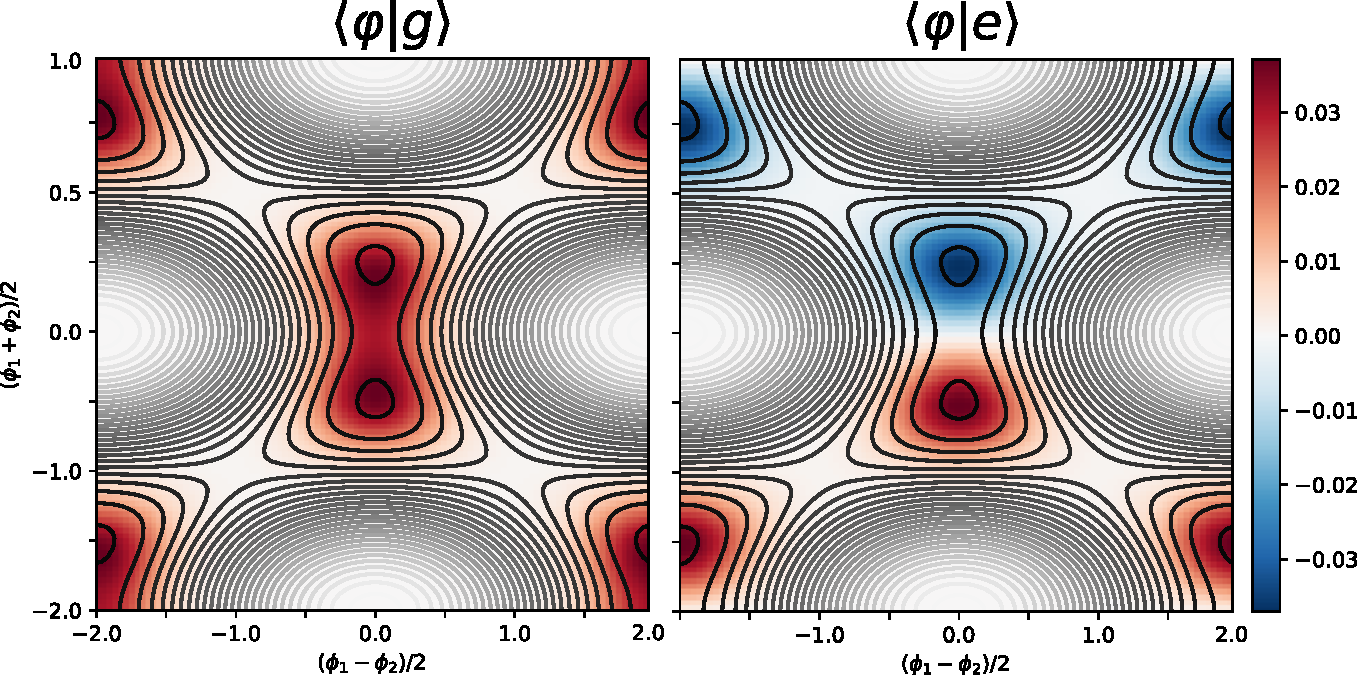
\includegraphics[width=0.95\textwidth]{images/3jj_vs.pdf}
	\caption{Волновая функция основного и первого возбужденного состояний потокового кубита при $\Phi=\Phi_0/2$. Линии уровня отображают потенциальную энергию.}
	\label{img: 3jj_vs}
\end{figure}
Высота барьера между двумя потенциальными ямами определяется параметром $\alpha$, и при $\alpha=0.5$ барьер исчезает. Поэтому данный параметр значительно влияет на собственные значения энергии и должен определяться достаточно точно, что может оказаться сложной задачей, особенно при использовании маленьких джозефсоновских переходов размерами порядка 200$\times$200 нм. Поэтому, как правило, воспроизводимость потоковых кубитов оказывается недостаточно хорошей, что в некоторой степени ограничивает их использование в качестве элемента многокубитных систем. Также очевидно, что вне точки $\Phi=\Phi_0/2$ кубит восприимчив к потоковому шуму, что неизбежно будет вызывать дефазировку. Тем не менее, потоковый кубит остается достаточно интересен, прежде всего, за счет большого ангармонизма по сравнению с трансмоном, речь о котором пойдет ниже.  
\subsection{Трансмон} Рассмотренный в разделе \ref{charge_q} зарядовый кубит обладал многими несовершенствами. Попытки развития и соверщенствования даннго кубита привели к созданию кубита-трансмона. Трансмон --- это зарядовый кубит, шунтированный большой емкостью, у которого $E_C \ll E_J$~(обычно в 50 раз и более). Идея создания такого кубита впервые появилась в \cite{cottet2002implementation}, позднее было проведено подробное теоретическое исследование данных кубитов \cite{koch2007charge} и практически сразу же последовали первые эксперименты c трансмонами \cite{transmon}. Для того, чтобы проиллюстрировать необходимость такой модификации, приведем на Рис.~\ref{img: disp_vs_anh} относительный  aнгармонизм трансмона $(\omega_{10}-\omega_{21})/\omega_{10}$ и относительное изменение частот нижних переходов трансмона при изменении наведенного заряда $n_g$, то есть величину $|\omega_{i0}(n_g=e)-\omega_{i0}(n_g=0)|/\omega_{i0}(n_g=0)$ .  для различных значений отношения $E_C/E_J$. При уменьшении этого отношения уменьшается ангармонизм кубита.
\begin{figure}[h]\center
	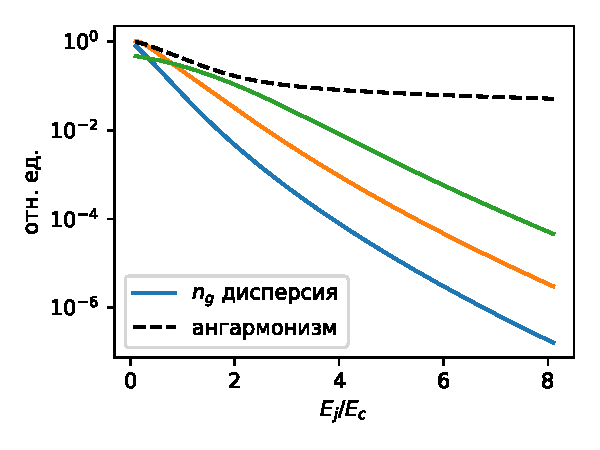
\includegraphics[width=0.75\textwidth]{images/disp_vs_anh.pdf}
	\caption{Изменение относительной зарядовой дисперсии для переходов 0-i трансмона и изменение ангармонизма основного перехода 0-1 в зависимости от отношения $E_J/E_C$. $E_C/h = 2$~ГГц}
	\label{img: disp_vs_anh}
\end{figure}
Для значений $E_C/E_J \approx 5$ кубит становится более похожим на гармонический осциллятор с относительно слабой нелинейностью в 5-10\% --- казалось бы, в таком эффекте нет никакой практической пользы. Но основным положительным эффектом от уменьшения $E_C/E_J$ является экспоненциально резкое падение зависимости энергетических уровней от $n_g$ --- так называемой зарядовой дисперсии. Особенно резко она уменьшается именно для низколежащих уровней, которые и используются на практике в качестве уровней кубита. Таким образом, удается достичь такого режима, когда ангармонизм еще достаточно большой и во многих ситуациях можно пренебречь верхними уровнями (или учесть их слабое влияние на динамику заселенности двух нижних уровней), и в то же время нежелательная зарядовая чувствительность практически подавлена. По этой причине для трансмонов характерны большие времена релаксации и декогеренции по сравнению как с зарядовыми, так и с потоковыми кубитами. Использование трансмонов при создании многокубитных схем оказалось весьма плодотворным, так как удалось разработать универсальные процессоры из 10 и более кубитов с полным контролем квантовых состояний. Однако, необходимо отметить, что во многих задачах трансмон нужно рассматривать как слабо нелинейный гармонический осциллятор, учитывая таким образом вклад верхних уровней. Например, при быстрых однокубитных операциях с трансмоном серьезную проблему представляют утечки заселенности кубита на второй возбуждённый уровень, которые необходимо предотвращать при помощи специальной коррекции управляющих импульсов. 

\subsection{вч-СКВИД в квантовом режиме}
Высокочастотный СКВИД - это прибор, представляющий собой джозефсоновский переход, шунтированный линейной индуктивностью $L$. Данный прибор изначально был предложен в 1965 г. для высокоточных измерений магнитного поля. Рассмотрим электрическую цепь вч-СКВИДа в квантовом режиме, см. Рис. Гамильтониан цепи имеет вид:
\begin{equation}
H = E_C \frac{n^2}{2} - E_J\cos(\phi - 2\pi\frac{\Phi}{\Phi_0}) + E_L\frac{\phi^2}{2}
\label{eq: rf_squid_ham}
\end{equation}
Зарядовая энергия возникает в результате внутренней емкости перехода и, возможно, некоторой паразитной емкости, которой обладает индуктивность из-за своего большого размера.
Динамика фазовой переменной $\varphi$ аналогична динамике координаты квантовой частицы, помещенной в параболический потенциал, модулированный гармонической функцией. При этом масса частицы обратно пропорциональна емкости. Большая емкость локализует систему в одной из потенциальных ям, малая же емкость приводит к тому, что собственные состояния имеют достаточно большую неопределенность по фазе. Особый интерес представляет режим, когда $E_L \ll E_C < E_J$. В этом случае образуется несколько низколежащих потенциальных ям практически с одинаковой энергией, и соответствующие состояния гибридизуются, см. Рис. \ldots. Получаемая при этом структура уровней сильно зависит от внешнего магнитного потока. Было показано, что в таком кубите возможно подавление квазичастичной релаксации, что было использовано для достижения времен жизни в несколько милисекунд. Однако, времена когерентности до недавнего времени оставались на уровне единиц микросекунд, и лишь в последнее время удалось повысить их до уровня кубитов-трансмонов \cite{grunhaupt2019granular}. 
\section{Микроволновая квантовая оптика}
\label{sec: microwave qo}

В этом разделе будет обсуждаться квантовооптические эффекты, возникающие при взаимодействии отдельных сверхпроводниковых кубитов с микроволновым излучением. За исключением некоторых общих вопросов, преимущественно будет рассматриваться кубит, встроенный в волновод и сильно связанный с модами излучения в этом волноводе. Одной из особенностей, нехарактерных для <<природных>> атомов, является возможность эффективной передачи квантового состояния кубита в волновод. Это дает возможность собрать излучение от кубита и анализируя его, наблюдать фундаментальные явления, такие как резонансная флуоресценция, электромагнитно-индуцированная прозрачность, керровскую нелинейность одиночного атома и многие другие любопытные физические эффекты. 
\subsection{Кубит как открытая квантовая система. Релаксация и дефазировка}
\label{sec:Lind}
До сих пор мы рассматривали кубит как изолированную квантовую систему. Однако, в реальной физической ситуации кубит будет взаимодействовать с бесконечным количеством других квантовых систем. К примеру, значительное влияние на кубит оказывают так называемые \textit{двухуровневые дефекты} --- локализованные спины, возникающие из-за различных примесей или вакансий в кремниевой подложке. Такое окружение является практически неуправляемым и имеет бесконечно большое число степеней свободы. Поэтому составить и тем более решить уравнения движения для сложной системы <<кубит+окружение>> не представляется возможным. Необходимо использовать специально разработанные методы приближенного описания динамики относительно простой квантовой системы (в данном случае кубита) в произвольном окружении с макроскопически большим числом степеней свободы.

Принципиальный подход учета влияния окружения $B$ на квантовую систему $S$ состоит в следующем. Составная система $S+B$ описывается матрицей плотности $\rho(t)=\rho_B(t)\otimes\rho_S(t)$, которая меняется во времени по эволюционному закону. Если же мы хотим выделить и описать процессы, происходящие c $S$, то можно ввести некоторое динамическое отображение $V(t)$, преобразующее матрицу плотности по закону $\rho_S(t) = V(t)\rho_S(0)$. Разумеется, его можно получить из закона унитарной эволюции полной системы при помощи взятия следа по переменным окружения, но как было сказано выше, этот закон достаточно сложен, и скорее всего, неизвестен. Поэтому нужно получить явный вид $V(t)$ из некоторых предположений о характере взаимодействия системы и окружения.

Предположим, что система взаимодействует с окружением через некоторые операторы $\hat{A}_i$, то есть, гамильтониан взаимодействия содержит эти операторы, действующие на переменные системы, в составе тензорного произведения с какими-то операторами окружения. Для сверхпроводящих кубитов во многих случаях справедливо \textit{Марковское приближение}. Его суть в том, что окружение предполагается состоящим из макроскопически большого числа  взаимодействующих между собой квантовых систем. Поэтому можно считать корреляционное время окружения гораздо меньшим чем характерное время распада квантового состояния отдельного кубита. В этом приближении можно показать, что динамика системы описывается так называемым Линбладовским уравнением:
\begin{equation}
\frac{d}{dt}\rho_S = \mathcal{L}\rho_S(t) = -\frac{i}{\hbar}[H, \rho_S] + \sum_{i=0}^{N^2-1}\gamma_i\big( A_i\rho_SA^\dag_i -\frac{1}{2}\{ A_iA^\dagger_i, \rho_S\}\big)
\label{eq: Master_L}
\end{equation}
Второй член уравнения, представленный в виде суммы, называется \textit{диссипатором} и обозначается $\mathcal{D}\rho_S$. Операторы $A_i$ называются операторами Линблада для различных каналов распада системы, а $\gamma_i$ --- скорости распада системы по различным каналам, они имеют размерность обратного времени зависят от силы связи и от корреляционных функций окружения. Это уравнение дает возможность учесть различные механизмы влияния окружения на кубит. На примере одиночного кубита рассмотрим основные каналы распада квантового состояния. 

\subsubsection{Релаксация кубита}
Кубит с гамильонианом $\frac{\hbar \omega}{2}\hat{\sigma}_z$ может взаимодействовать с окружением посредством обмена квантами возбуждения, или энергией. Такое взаимодействие описывается гамильтонианом типа $H_{int} =\gamma(\hat{\sigma}_- \hat{a}^\dag + \hat{\sigma}_+ \hat{a})$. Используя \eqref{eq: Master_L}, получим выражение для диссипатора:
\begin{equation}
\mathcal{D}\rho_S(t) = \gamma\left( \sigma_- \rho_S(t) \sigma_+ -\frac{1}{2}\sigma_-\sigma_+\rho_S(t) -\frac{1}{2}\rho_s(t)\sigma_-\sigma_+ \right),
\label{eq: diss_ops}
\end{equation}
, или в явной матричной записи:
\begin{equation}
\mathcal{D}\rho_S = \frac{1}{2}\left[\begin{matrix}\gamma \left(- \rho_{z}{\left (t \right )} - 1\right) & \frac{\gamma}{2} \left(- \rho_{x}{\left (t \right )} + i \rho_{y}{\left (t \right )}\right)\\\frac{\gamma}{2} \left(- \rho_{x}{\left (t \right )} - i \rho_{y}{\left (t \right )}\right) & \gamma \left(\rho_{z}{\left (t \right )} + 1\right)\end{matrix}\right],
\label{eq: diss}
\end{equation}
где $\rho_x, \rho_y, \rho_z$ - компоненты блоховского вектора, введенного в \eqref{eq: rho_to_bloch}. Диагональные члены полученной матрицы показывают, что диссипация в первую очередь вызывает плавное <<перетекание>> заселенности состояния $\ket{1}$ в состояние $\ket{0}$, а недиагональные члены выражают тот факт, что любой канал распада состояния кубита со скоростью $\gamma$ также вносит дефазировку когерентностей кубита со скоростью $\gamma/2$. 
\subsubsection{Чистая дефазировка}
Еще один способ взаимодействия с окружением --- это влияние на резонансную частоту кубита, например, взаимодействие типа $H_{int} = \gamma_{\phi}\hat{a}^\dag\hat{a}\hat{\sigma}_z$. Это взаимодействие может реализовываться, например, в дисперсионном режиме модели Джейнса-Каммингса (см. ниже), когда перебросы двухуровневых систем в подложке эффективно вызывают сдвиг частоты перехода кубита. Более сложные механизмы дефазировки, связанные с вовлечением виртуальных двухфотонных процессов, описываются в \cite{Carmichael}. При этом результирующий диссипатор имеет вид:
\begin{equation}
\mathcal{D}\rho_S(t) = \frac{\gamma_\phi}{2}\left( \sigma_z\rho_S(t)\sigma_z - \rho_S(t)\right) = \frac{\gamma_\phi}{2}\left[\begin{matrix}0 & - \rho_{x}{\left (t \right )} - i \rho_{y}{\left (t \right )}\\-  \rho_{x}{\left (t \right )} + i \rho_{y}{\left (t \right )} & 0\end{matrix}\right]
\end{equation}
Недиагональные члены этого диссипатора вызывают затухание когерентностей кубита со скоростью $\gamma_\phi/2$, при этом никак не изменяются диагональные члены матрицы плотности. 
\subsection{Взаимодействие искусственного атома с внешним полем. Гамильтониан Джейнса-Каммингса.}
Рассмотрим, как одиночный естественный атом, расположенный в открытом пространстве, взаимодействует с падающим на него монохроматическим излучением. Будем работать в т.н. \textit{дипольном приближении}, которое предполагает, что длина волны электромагнитного поля гораздо больше размеров атома. Для случая сверхпроводникового кубита размерами 10-100 мкм это приближение выполняется для любых частот гигагерцового диапазона. Гамильтониан взаимодействия кубита и атома можно записать как $H_{int} = - \mathbf{d}\cdot\mathbf{E}$
где $\mathbf{d}$ --- оператор дипольного момента сверхпроводникового искусственного атома. Мы в данном случае предположили что атом связывается с напряженностью $\mathbf{E}$ электрического поля в точке расположения атома. Дипольный момент записывается как $\mathbf{d} = e \braket{g|\mathbf{r}|e}(\sigma_+ + \sigma_-)$, 
а стандартная процедура квантования поля дает для $\mathbf{E}$ следующее выражение: $$\mathbf{E} = \frac{1}{(2\pi)^3}\int\limits_{\omega}^{}\sqrt{\frac{\hbar\omega}{2\varepsilon_0}} \left(a_\omega^\dag+a_\omega\right).$$
После подстановки этих выражений в гамильтониан взаимодействия и учета гамильтонианов кубита и поля получается гамильтониан Раби:
\begin{equation}
H_R = \int\limits_{\omega}^{}\hbar \omega a^\dag_\omega a_\omega + \frac{1}{2}\hbar \omega_q\sigma_z + \hbar\int\limits_{\omega}^{}g_{\omega}(a_\omega^\dag + a_\omega)(\sigma_-+\sigma_+).
\end{equation}
Интегрирование здесь и ранее ведется по континууму мод, которые могут распространяться в волноводе. Если предположить, что константы связи $g_\omega$ достаточно малы по сравнению с частотой кубита, то справедливо приближение вращающейся волны. При переходе во вращающуюся систему отсчета с помощью унитарного преобразования $U_R =\exp\left({-i/2\hbar}(\omega_q\sigma_z+\omega a^\dag a)\right) $ слагаемые $a^\dagger\sigma_+$ и $a\sigma_-$ приобретут быстроосциллирующие множители $\exp\left( \pm(\omega+\omega_q)t\right)$. Эти множители практически не вносят вклада в динамику системы, поскольку:
$$\int_{}^{}e^{\pm in \omega t} dt=\frac{e^{\pm in \omega t}}{\pm in\omega}\propto \frac{1}{\omega}.$$
Отбрасывая эти слагаемые, получаем гамильтониан Джейнса-Каммингса:
\begin{equation}
H_{J-C} = \int\limits_{\omega}^{}\hbar \omega a^\dag_\omega a_\omega + \frac{1}{2}\hbar \omega_q\sigma_z + \hbar\int\limits_{\omega}^{}g_{\omega}(a_\omega^\dag\sigma_- + a_\omega\sigma_+).
\end{equation}
Отметим, что для распространения волны частотой 1-10 ГГц в копланарной проходной линии в случае, когда длина волны много превышает размер зазора, возможна только одна поляризация, при которой электрическое поле лежит в плоскости линии и направлено от центральной жилы к заземленным плоскостям (в течение одного полупериода колебаний). Все остальные моды, в том числе т.н. \textit{нечетные} моды, при которых ток течет по краям центральной жилы в противоположные стороны, а электрическое поле по обе стороны центральной жилы направлено в одну сторону, имеют гораздо более высокую частоту и не возбуждаются в интересующем нас диапазоне.   

\subsection{Режим сильной связи}
Понятие режима сильной связи можно применить к любым двум квантовым системам, которые взаимодействуют между собой. Для любых таких систем можно записать гамильтониан, который будет содержать часть, описывающую взаимодействие. Любое взаимодействие сводится к некоторой эффективной константе связи $g$, имеющей размерность энергии (частоты). При этом, помимо взаимодействия друг с другом, каждая из систем имеет некоторые потери энергии и/или дефазировку за счет взаимодействия со своим окружением, и эти потери тоже характеризуются некоторыми константами $\{\Gamma\}$. Для изучения совместной квантовой динамики систем наиболее интересным представляется случай, когда $g \gg \Gamma_i \in \{\Gamma\}$, то есть, сила взаимодействия значительно превосходит все возможные <<паразитные>> процессы, вызванные окружением и приводящие к потере квантового состояния в каждой из систем. В таком случае говорят, что эти системы находятся в режиме сильной связи. В случае атома, сильно связанного с электромагнитным полем внутри резонатора или проходной линии, возникает ряд интересных физических явлений, например, вакуумное Раби-расщепление 

Рассмотрим одномодовый случай модели Джейнса-Каммингса, который реализуется в случае связи кубита и резонатора. Покажем, что эта модель допускает точное решение. Естественный базис совместного гильбертова пространсва состояний кубита и резонатора $H_Q \otimes H_R$ можно составить из функций $\ket{\{e,g\}; n}, n \in \mathcal{N}$, в котором гамильтониан примет блочно-диагональный вид:
\begin{equation}
H_{JC}/\hbar=
\kbordermatrix{ \mathrm{state} &  \ket{e, n-1} & \ket{g, n} \\
	\ket{e, n-1} & \omega_q + (n-1)\omega & g \sqrt{n} \\
	\ket{g, n} & g\sqrt{n} & n\omega }
\end{equation}
Состояния гибридизуются попарно, и результирующие собственные энергии и состояния модели выглядят следующим образом:
\begin{equation}
\begin{split}
\ket{-,n} &= \cos \theta_n\ket{g,n}-\sin\theta_n\ket{e, n-1},\\
\ket{+,n} &= \cos \theta_n\ket{g,n}+\sin \theta_n \ket{e, n-1}, \text{где}\\
\theta_n &= \frac{1}{2}\arctan\Big(\frac{2g\sqrt{n}}{\Delta}\Big)
\end{split}
\end{equation}
\subsection{Эластичное и неэластичное рассеяние в копланарной линии}
\label{sec: scatt}
В этом разделе будет рассмотрен процесс взаимодействия кубита и электромагнитный волны, распространяющейся в копланарной проходной линии вдоль оси $x$. Несмотря на кажущуюся простоту задачи, физическая суть происходящих при этом рассеянии явлений достаточно сложна. Будет показано, что есть принципиально различные компоненты рассеянного кубитом  сигнала: \textit{эластичная} и \textit{неэластичная} компонента. Для этого необходимо будет записать и решить уравнения динамики кубита с учетом релаксации в линию и проанализировать полученное стационарное решение. 
\subsubsection{Классическое поле в линии}   Начнем с классического описания взаимодействия некоторой системы, связанной с электромагнитным полем в линии. По сути, будет рассматриваться классический вариант \textit{теории входа-выхода}. Линия обладает погонной емкостью $c$ и погонной индуктивностью~$l$. Распространяющая волна создает некоторое распределение тока и напряжения вдоль линии. Уравнения, описывающие это распределение, называются \textit{телеграфными уравнениями} и записываются следующим образом:
\begin{equation}
\begin{split}
\frac{\partial V(x,t) }{\partial x} = -l\frac{\partial I(x,t)}{\partial t},\quad
\frac{\partial I(x,t) }{\partial x} = -c\frac{\partial V(x,t)}{\partial t}
\label{eq: telegr}
\end{split}
\end{equation}
Для удобства можно также разделить волны, распространяющиеся направо и налево в линии, сопоставив им соотвествующие напряжения $V^\rightarrow(x,t)$ и  $V^\leftarrow(x,t)$. Тогда полное напряжение и ток в линии записываются как:
\begin{equation}
\begin{split}
V(x,t) &= V^\rightarrow(x,t) + V^\leftarrow(x,t) \\
I(x,t) &= \frac{1}{Z}(V^\rightarrow(x,t) - V^\leftarrow(x,t)),
\label{eq: dirs}
\end{split}
\end{equation}
где $Z = \sqrt{l/c}$ - волновое сопротивление линии. Волновые уравнения принимают вид:
\begin{equation}
\begin{split}
	v\frac{\partial V^\rightarrow(x,t)}{\partial x} = -\frac{\partial V^\rightarrow(x,t)}{\partial t}, 
	v\frac{\partial V^\leftarrow(x,t)}{\partial x} = \frac{\partial V^\leftarrow(x,t)}{\partial t}, 
	\label{eq: telegr_dirs}
\end{split}
\end{equation}
где $v = 1/\sqrt{lc}$ - скорость распространения волны. 
Часто встречается случай, когда полубесконечная линия при $x>0$ замыкается на некоторую электрическую схему $S$, например, сверхпроводниковый кубит, расположенный в точке $x=0$. Тогда по отношению к этой схеме можно рассматривать возможные решения \eqref{eq: telegr_dirs} как входное и выходное напряжение, соответственно: $V^\leftarrow(t-x/v) \equiv V_{in}(t-x/v)$ и $V^\rightarrow(t+x/v) \equiv V_{out}(t+x/v)$. Используя \eqref{eq: dirs}, можно получить связь входного и выходного напряжений: 
\begin{equation}
V_{out}(t) = V_{in}(t) + ZI(0,t)
\label{eq: in_out}
\end{equation}
 Для того, чтобы эти уравнения полностью определяли ток и напряжение в линии, к ним необходимо добавить граничные условия, соответствующие реальной физической задаче.
\begin{itemize}
	\item  Если никакой системы нет и в точке $x=0$ линия претерпевает разрыв, то $I(0,t)=0$. Поэтому из \eqref{eq: in_out} следует идеальное отражение волны: $V_{out}(t) = V_{in}(t)$.
	\item Если отсутствует входной сигнал, то получаем $V_{out}(t) = ZI(0,t)$. Полубесконечная линия представляет из себя резистор с сопротивлением $Z$, подключенный к системе в качестве нагрузки. Измеряя напряжение $V_{out}(t)$, можно изучать динамику распада системы.
	\item В наиболее общем случае $I(0,t)\ne 0$, и схема инжектирует ток в линию. При 
	0
	необходимости можно рассчитать напряжение в точке $x=0$: $V(0,t) = 2V_{in}(t) + ZI(0,t)$.  	
\end{itemize}
\subsubsection{Взаимодействие кубита с классическим полем в линии}
Рассмотрим отдельный сверхпроводящий кубит, подключенный к бесконечной линии в точке $x=0$ при помощи связывающей емкости, см. Рис.~\ref{fig: el_scheme}.
\begin{figure}[h]
	\centering
	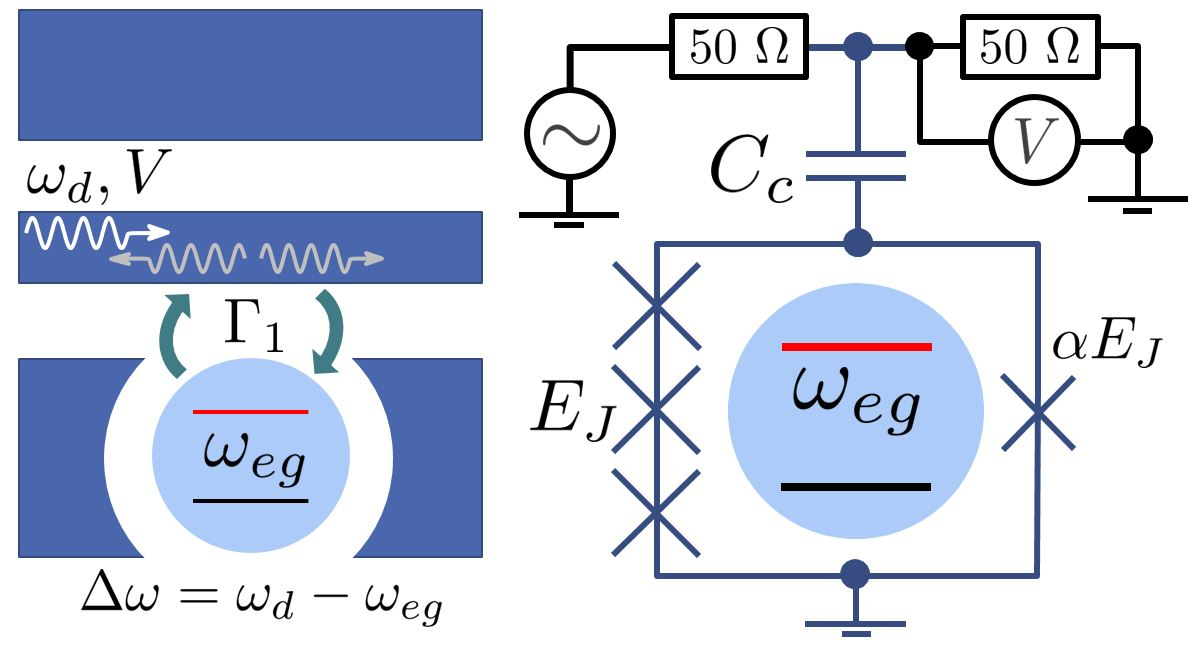
\includegraphics[width=0.9\textwidth]{qubit_electr_scheme.jpg}
	\caption[Эквивалентная электрическая схема подключения кубита к волноводной линии]{Слева: принципиальная схема кубита в открытом одномерном пространстве. Справа: эквивалентная электрическая схема, описывающая кубит, емкостно связанный с копланарным волноводом.}
	\label{fig: el_scheme}
\end{figure}
Применим к нему классическую теорию входа-выхода, изложенную также в~\cite{zagoskin2011quantum}. Это даст возможность получить аналитическое выражение для эластично рассеянного поля. 

Согласно схеме подключения кубита, появляется дополнительный узел электрической цепи, через который в линию будет втекать дополнительный ток из кубита. Таким образом, граничные условия можно записать в виде:
\begin{equation}
\begin{split}
	V(-0,t) &= V(+0,t) \\
	I(-0,t) + C_c\frac{d \langle \hat{V}_q \rangle }{dt} &= I(+0,t)
	\label{eq: bound_cond}
\end{split}
\end{equation}
Из граничных условий видно, что напряжение в точке $x\!=\!0$ меняется непрерывно, тогда как ток претерпевает скачок. Поэтому удобно рассмотреть ситуацию, когда распространяющаяся слева направо электромагнитная волна, амплитуда напряжения в которой равна $V_0$, претерпевает рассеяние на кубите. Запишем напряжение слева и справа от кубита в виде:
\begin{equation}
\begin{split}
V(x>0,t) &= t V_0 e^{-i(\omega t - k x)} \\
V(x<0,t) &= V_0 e^{-i(\omega t - k x)} - r V_0 e^{-i(\omega t + k x)} 
\label{eq: wave_scattering}
\end{split}
\end{equation}
Из этих уравнений с учетом условий \eqref{eq: bound_cond} получаем, что $t=1-r$. Подставляя \eqref{eq: wave_scattering} во второе уравнение в \eqref{eq: telegr} и интегрируя по координате $x$, получаем уравнения для тока:
\begin{equation}
\begin{split}
I(x<0,t) &= c V_0 \frac{\omega}{k}\cdot \big( re^{-i(\omega t + k x)} + e^{-i(\omega t - k x)}\big)\\
I(x>0,t) &= c V_0 \frac{\omega}{k} \cdot te^{-i(\omega t - k x)}
\end{split}
\label{eq: cur}
\end{equation}
Комбинируя эти выражения с уравнением для тока из \eqref{eq: bound_cond}, получим еще одно соотношение для коэффициентов прохождения и отражения:
\begin{equation}
1 + r = t + C_c\frac{k}{\omega cV_0}\frac{d \langle \hat{V}_q \rangle }{dt}e^{i\omega t}.
\end{equation}
Учитывая что $\omega/k=v=1/\sqrt{lc}$ - скорость распространения света в линии, получаем окончательное выражение для коэффициента отражения:
\begin{equation}
r = \frac{Z}{2V_0}C_c\frac{d\langle\hat{V}_q\rangle}{dt} e^{i\omega t}
\label{eq: r_derived}
\end{equation}  
\subsubsection{Основное квантовое уравнение кубита под действием резонансного поля}
Амплитудные коэффициенты отражения и прохождения достаточно удобны для их непосредственного измерения. Однако, полученное выражение \eqref{eq: r_derived} для $r$ и аналогичное выражение для $t$ непригодны для подгонки практических результатов, так как остается необходимым проанализировать операторный множитель и выразить его через измеряемые характеристики системы. 

Для простоты рассмотрим случай зарядового кубита в точке вырождения $\theta=\pi/2$ . Оператор напряжения на связывающем конденсаторе пропорционален заряду кубитного острова $\langle \dot{V_q} \rangle=\langle \dot{q} \rangle/C_\Sigma$, где $C_\Sigma$ - суммарная емкость между островом и землей. 
Согласно \eqref{eq: charge_e}, собственные состояния кубита в точке вырождения выражаются через зарядовые состояния как $\ket{g} = (\ket{0}+\ket{1})/\sqrt{2}$ и $\ket{e} = (\ket{0}-\ket{1})/\sqrt{2}$, поэтому в матричном виде можно записать:
\begin{equation}
\hat{q} = 
\begin{bmatrix}
\braket{e|\hat{q}|e} & \braket{e|\hat{q}|g} \\
\braket{g|\hat{q}|e} & \braket{g|\hat{q}|g}
\end{bmatrix} = e
\begin{bmatrix*}[r]
 0 &-1 \\
-1 & 0
\end{bmatrix*} + e
\begin{bmatrix*}[r]
1 & 0 \\
0 & 1
\end{bmatrix*}, 
\end{equation}
значит, $\braket{\dot{q}}=e\frac{d\braket{\sigma_x(t)}}{dt}$. Усреднение в данном случае означает математическое ожидание оператора по состоянию кубита. Поскольку кубит бесконечно долго взаимодействует с непрерывной волной и при этом одновременно излучает в линию, то логично предположить, что эти процессы компенсируют друг друга. Поэтому с течением времени кубит должен оказаться в некотором стационарном состоянии, которое можно определить из условия $\dot{\rho} = 0$. Для нахождения $\langle\sigma_x(t)\rangle$ необходимо записать и решить основное квантовое уравнение для кубита. Гамильтониан взаимодействия зарядового кубита с напряжением в линии имеет вид:
\begin{equation}
H_{int} = C_cV\hat{V}_q = \frac{C_c}{C_\Sigma}V_0\cos(\omega_d t + \varphi)\braket{g|\hat{q}|e}\sigma_x,
\label{eq: Hint_class}
\end{equation} 
причем для зарядового кубита $\braket{g|\hat{q}|e} = e$. Для случая трансмона \cite{koch2007charge} собственные состояния являются суперпозициями большого числа зарядовых состояний, поэтому рассчитать матричный элемент несколько сложнее: 
\begin{equation}
\braket{g|\hat{q}|e} = \frac{2e}{\sqrt{2}}\left(\!\frac{E_J}{E_C}\!\right)^{\!\frac{1}{4}}.
\end{equation}
Вводя обозначение для емкостного коэффициента эффективности связи  $\beta = C_c/C_\Sigma$ и Раби-частоты $\Omega = \beta V_0\braket{g|\hat{q}|e}/\hbar$, получаем из \eqref{eq: Hint_class} окончательное выражения для гамильтониана взаимодействия. Полный гамильтониан примет вид:
\begin{equation}
H = H_q + H_{int} = -\frac{\hbar \omega_q}{2}\hat{\sigma}_z+ \hbar\Omega\cos(\omega_d t + \varphi)\hat{\sigma}_x
\label{eq: H_int_class_final}
\end{equation} 
Чтобы вывести основное квантовое уравнение, сначала воспользуемся приближением вращающейся волны, описанным в разделе \ref{sec: qubit}. Преобразуя $H$ при помощи унитарного преобразования $U=\exp(-i\omega_d\sz/2\hbar)$, имеем:
\begin{equation}
\label{eq: Hrot}
H_{rwa}=UHU^\dagger-i\dot{U}U^\dag \approx \frac{\hbar}{2}\left[\begin{matrix}- \omega_d + \omega_q & \Omega e^{- i \varphi}\\\Omega e^{i \varphi}  & \omega_d - \omega_q\end{matrix}\right],
\end{equation}
где были отброшены быстро осциллирующие члены $\Omega e^{\pm i \varphi} e^{\pm2 i \omega_d t}$ в недиагоальных слагаемых. Используя этот гамильтониан, можно записать основное квантовое уравнение, представляющее собой уравнение Лиувилля-фон Неймана для эволюции квантовой системы, описывающейся оператором плотности и линбладовский член, характеризующий взаимодействие с внешней средой:
\begin{equation}
\frac{d\rho}{dt} = -\frac{i}{h}[H_{rwa}, \rho] + \mathcal{L}.
\label{eq: QLiouv}
\end{equation}
Линдбладовский член, который включает в себя релаксацию $\Gamma_1$ и дефазировку $\gamma_\phi$, описанные ранее в разделе \ref{sec:Lind}, имеет следующий вид:
\begin{equation}
\mathcal{L} = \left[\begin{matrix}-\Gamma_1 \left(\rho_{z}+1\right) & -\Gamma_1 \left( \frac{\rho_{x}}{2}-\frac{i \rho_{y}}{2}\right) - \gamma_{\phi} \left(\rho_{x} - i \rho_{y}\right)\\-\Gamma_1 \left( \frac{\rho_{x}}{2} + \frac{i \rho_{y}}{2}\right) - \gamma_{\phi} \left(\rho_{x} + i \rho_{y}\right) & \Gamma_1 \left(\rho_{z} + 1\right)\end{matrix}\right]
\end{equation}
После преобразований уравнение запишется в следующем виде:
\begin{equation}
\label{eq: Bloch}
\dot{\vec{\sigma}}{\left(t\right)} = \mathbf{M}\vec{\sigma}{\left(t\right)} + \vec{b}, 
\end{equation}
где введены обозначения:
\begin{equation}
\vec{\sigma}(t) = \left[\begin{matrix}\rho_x(t)\\\rho_y(t)\\\rho_z(t)\end{matrix}\right], \:	
\mathbf{M}=\left[\begin{matrix}- \frac{\Gamma_1}{2} - \gamma_{\phi} & \omega_d - \omega_q & \Omega \sin{\varphi}\\- \omega_d + \omega_q & - \frac{\Gamma_1}{2} - \gamma_{\phi} & - \Omega \cos{\varphi }\\- \Omega \sin{\varphi } & \Omega \cos{\varphi} & - \Gamma_1\end{matrix}\right], \:\vec{b} = \left[\begin{matrix}0\\0\\- \Gamma_1\end{matrix}\right].
\end{equation}
Уравнения \eqref{eq: Bloch} называются \textit{уравнениями Блоха} и полностью описывают динамику двухуровневой системы, связанной с окружением и находящейся под действием внешнего электромагнитного поля. 
\subsubsection{Динамика состояния кубита под действием поля}
Уравнения Блоха \eqref{eq: Bloch} могут быть решены точно. Для получения решения воспользуемся подстановкой $\vec{\sigma}(t) = e^{\mathbf{M}t}\vec{v}(t)$, которая преобразует уравнение \eqref{eq: Bloch} к виду:
\begin{equation}
e^{\mathbf{M}t}\dot{\vec{v}}(t) = \vec{b},
\end{equation}откуда формальным интегрированием получаем: $\vec{v} = \mathbf{-M^{-1}}e^{-\mathbf{M}t}\vec{b} + \vec{v}_0$. Константа интегрирования $\vec{v}_0$ зависит от начального состояния атома: $\vec{\sigma}_0 =  -\mathbf{M^{-1}}\vec{b} + \vec{v}_0$. С учетом этого получаем окончательное выражение:
\begin{equation}
\vec{\sigma}(t) = -\mathbf{M^{-1}}\vec{b} + e^{\mathbf{M}t}\left(\vec{\sigma}_0 + \mathbf{M^{-1}}\vec{b}\right)
\end{equation}
Окончательные выражения, описывающие динамику атома, достаточно громоздки. Выпишем решение для частного случая $\varphi=0, \delta\omega=\omega_q - \omega_d = 0$:
\begin{equation}
\textstyle
\frac{1}{2 \left(2\Omega ^2+2 \gamma _{\varphi } \Gamma _1+\Gamma _1^2\right) \Omega _r}
\left[\begin{smallmatrix}
0 \\
4 \Omega  \Gamma _1 \Omega _r+e^{-\Gamma_r t } \Omega \left[  
	\left(4 \Omega ^2+2 \gamma _{\varphi } \Gamma _1-\Gamma _1^2\right)\sin \Omega _rt-4  \Gamma _1 \Omega _r\cos \Omega_rt\right] \\
-2 \Gamma _1 \left(2 \gamma _{\varphi }+\Gamma _1\right) \Omega _r-e^{-\Gamma_r t } \Omega
	^2 \left[\left(2 \gamma _{\varphi }+3 \Gamma _1\right)\sin \Omega _r t +4  \Omega _r \cos \Omega _r t\right] \\ 
\end{smallmatrix}
\right]
\label{eq: dyn_sol}
\end{equation}
Можно заметить, что динамика имеет вид осцилляций, которые затухают со временем, см.~Рис. \ref{img: Rabi_dyn_res}. Они называются осцилляциями Раби. 
\begin{figure}[t]
	\centering
	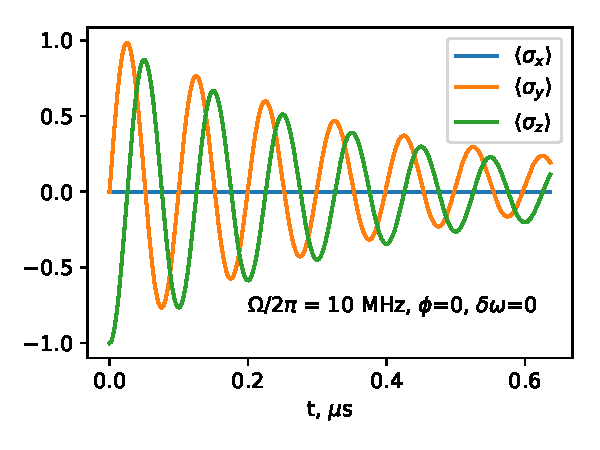
\includegraphics[width=0.6\textwidth]{images/Rabi_res.pdf}
	\caption[Динамика состояния кубита под действием внешнего поля в случае резонанса]{Динамика среднего состояния кубита под воздействием поля. Компоненты блоховского вектора $\{\braket{\sigma_x(t)}, \braket{\sigma_y(t)}, \braket{\sigma_z(t)}\}$ в явном виде заданы выражением $\eqref{eq: dyn_sol}$.}
	\label{img: Rabi_dyn_res}
\end{figure}

Отметим некоторые особенности полученного решения. Во-первых, частота Раби осцилляций определяется как $\Omega_r = \sqrt{\Omega^2-(\Gamma_1-2\gamma_\varphi)^2/16}$, и практически совпадает с $\Omega$ в случае достаточно сильного драйва. Затухание Раби-осцилляций определяется как $\Gamma_r = \frac{1}{4}\left(2 \gamma _{\varphi }+3 \Gamma _1\right) = \left(\Gamma_1 + \Gamma_2\right)/2$. Этот результат качественно объясняется тем, что примерно половину времени кубит проводит на экваторе сферы Блоха, где он существенно подвержен влиянию дефазировки, а другую половину кубит имеет положительную проекцию на ось $z$, и соответственно, подвержен влиянию затухания.
В случае $\delta\omega \ne 0$ окончательный ответ еще более громоздкий, поэтому мы не приводим уравнения, описывающие динамику в этом более общем случае. Динамика кубита при ненулевой отстройке изображена на~Рис.~\ref{img: Rabi_dyn_det} и \ref{img: Bloch_Rabi_dyn_det}. Заметим, что общий характер колебаний остается примерно таким же, что и в случае $\delta\omega=0$, однако, заметно меняется конечное состояние кубита, в котором он оказываеся после осцилляций - стационарное состояние. Получим явное выраджение, описывающее стационарное состояние кубита.
\begin{figure}[t]
	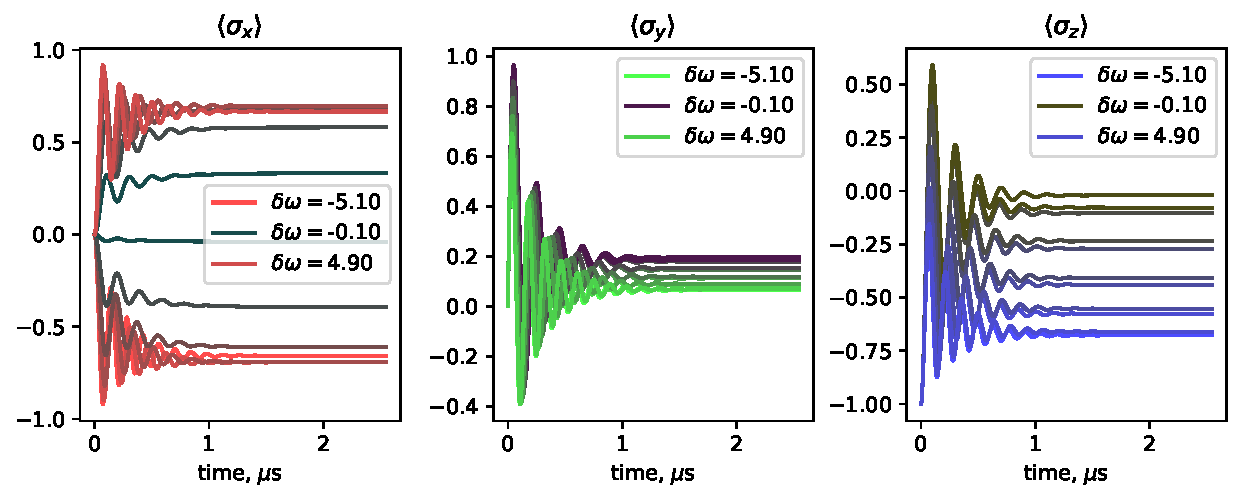
\includegraphics[width=0.98\textwidth]{images/Rabi_det_2.pdf}
	\caption[Динамика состояния кубита под действием внешнего поля: случай ненулевой отстройки]{Динамика компонент блоховского вектора $\vec{\sigma}(t)$ для $\Gamma_1=0.5, \gamma_\varphi=0.1, \Omega = 10$~МГц. Линии на каждом из графиков соответствуют значениям $\delta\omega=[-5.1,4.9]$~МГц }
	\label{img: Rabi_dyn_det}
\end{figure}
\begin{figure}[h]
	\centering
	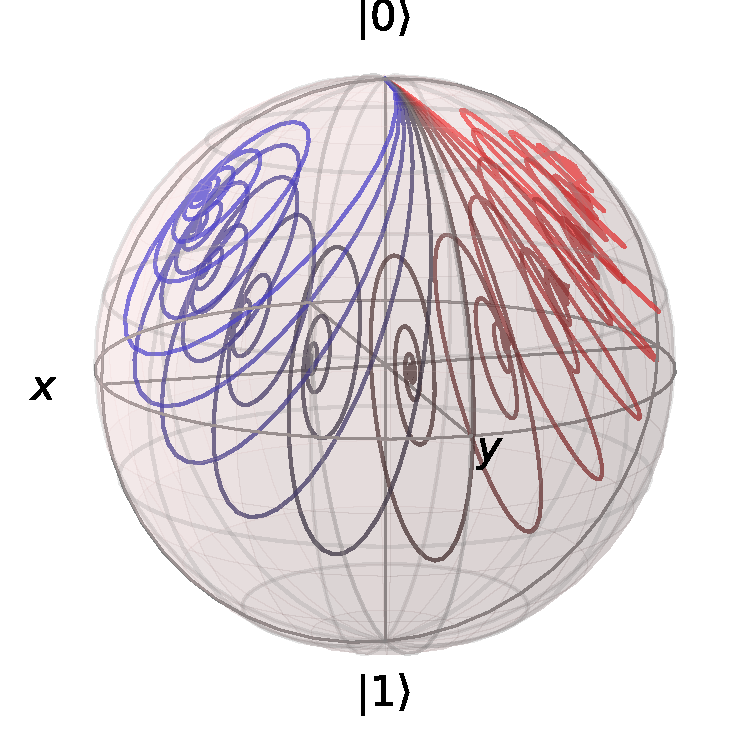
\includegraphics[width=0.65\textwidth]{images/Bloch_rabi_det.pdf}
	\caption[Динамика состояния кубита под действием внешнего поля на сфере Блоха]{Динамика состояния кубита при ненулевой отстройке внешнего драйва, изображенная на сфере Блоха. Кривые построены при тех же параметрах, которые использованы для Рис. \ref{img: Rabi_dyn_det}.}
	\label{img: Bloch_Rabi_dyn_det}
\end{figure}
\subsubsection{Стационарное решение уравнений Блоха}
Поскольку кубит постоянно взаимодействует с полем, время от времени обмениваясь энергией или информацией с внешней средой, то можно предположить, что временная динамика матрицы плотности, которая, строго говоря, описывает распределение эволюций одинаковых систем, через достаточно долгое время придет к некоторому стационарному значению $\vec{\sigma}_{st}$. Это легко проверить, положив в уравнениях \eqref{eq: Bloch}  $\dot{\vec{\sigma}}(t)=0$, что делает дифференциальные уравнения алгебраическими. Полагая $\varphi=0$ (что задает вращение вокруг оси $x$) и решая уравнения относительно компонент блоховского вектора, находим:
\begin{multline}
\rho_{x} = \frac{4 \Gamma_{1} \Omega \delta\omega}{4 \Gamma_{1} \delta\omega^{2} + \Gamma_{1} \left(\Gamma_{1} + 2 \gamma_{\varphi}\right)^{2} + 2 \Omega^{2} \left(\Gamma_{1} + 2 \gamma_{\varphi}\right)},\\\rho_{y} = \frac{2 \Gamma_{1} \Omega \left(\Gamma_{1} + 2 \gamma_{\varphi}\right)}{4 \Gamma_{1} \delta\omega^{2} + \Gamma_{1} \left(\Gamma_{1} + 2 \gamma_{\varphi}\right)^{2} + 2 \Omega^{2} \left(\Gamma_{1} + 2 \gamma_{\varphi}\right)},\\ \rho_{z} = - \frac{\Gamma_{1} \left(4 \delta\omega^{2} + \left(\Gamma_{1} + 2 \gamma_{\varphi}\right)^{2}\right)}{4 \Gamma_{1} \delta\omega^{2} + \Gamma_{1} \left(\Gamma_{1} + 2 \gamma_{\varphi}\right)^{2} + 2 \Omega^{2} \left(\Gamma_{1} + 2 \gamma_{\varphi}\right)},
\label{eq: stat_sol}
\end{multline}
где введено обозначение $\delta\omega=\omega_d-\omega_q$.
\begin{figure}[h]
	{ \raggedleft
		\hfill
		\def\svgwidth{2.5in}
		\fontsize{19pt}{19pt}\selectfont
		\subbottom[\label{img: bloch_stat1}]{%
			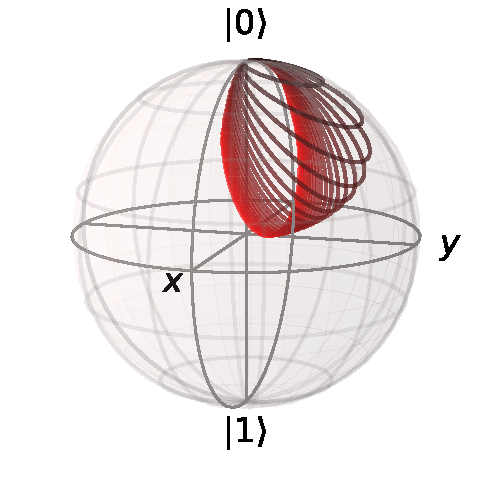
\includegraphics{images/bloch_stat1.pdf}}
		\hfill
		\def\svgwidth{2.5in}
		\subbottom[\label{img: bst2}]{%
			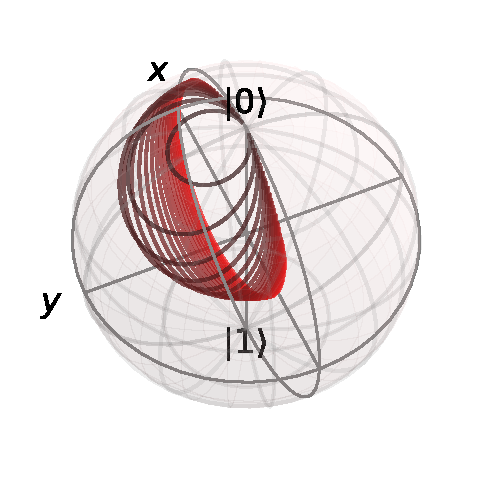
\includegraphics{images/bloch_stat2.pdf}}
		
		\hfill
	}
	\caption[Стационарное состояние кубита, вращаемого электромагнитным полем.]{Стационарное состояние \eqref{eq: stat_sol} кубита под воздействием поля, изображенное на сфере Блоха. Различные линии соответствуют значениям $\Omega=[0,10]$, $\Gamma_1=2, \gamma_\varphi=0 $~МГц. Каждая линия соответствуют изменению $\delta\omega=[-10,10]$~МГц. Панели а) и б) изображают одни и те же линии под различными ракурсами. Отметим, что эти линии образованы множеством точек, к которым приходит кубит после динамики, изображенной на~Рис. \ref{img: Bloch_Rabi_dyn_det} \label{img: bloch_stat}}
	
\end{figure}
Стационарные состояние в зависимости от параметров $\Omega, \Gamma_1, \gamma_\varphi$ изображено на Рис.~\ref{img: bloch_stat}. В случае $\Omega\!\ll\!\Gamma_1$ стационарное состояние приближено к состоянию $\ket{0}$, поскольку поле достаточно слабое для эффективного возуждения кубита. В случае $\Omega\!\gg\!\Gamma_1$ стационарное состояние приближено к смешанному состоянию, но имеет ненулевую проекцию на экваториальную плоскость. Рассчитаем эластичную часть излучения кубита в стационарном состоянии
\subsubsection{Эластичное рассеяние}
Поскольку нас интересует сигнал, рассеянный кубитом назад, то необходимо выразить компоненту поля, соответствующую отрицательной частоте, то есть, соотвествующую оператору $\langle\hat{\sigma}_- \rangle$. Используя решения \eqref{eq: stat_sol} и возвращаясь в лабораторную систему отчета, получим:
\begin{equation}
\braket{\hat{\sigma}_-} = \frac{1}{2}\left(\rho_x-i\rho_y\right) = -\frac{\Omega/2\Gamma_2}{1+(\delta\omega/\Gamma_2)^2+\Omega^2/\Gamma_1\Gamma_2}\left(\frac{\delta\omega}{\Gamma_2}-i\right)e^{-i\omega_d t},
\label{eq: stat_s-}
\end{equation} 
где $\Gamma_2 = \Gamma_1/2
 + \gamma_\varphi$~ обозначает полную дефазировку кубита. Выражение \eqref{eq: stat_s-} уже может быть подставлено в \eqref{eq: r_derived}, однако, перед тем как сделать это, необходимо рассмотреть явную связь между излучательной релаксацией $\Gamma_1$ кубита в линию и квантовыми флуктуациями электромагнитного поля в линии, вызывающими эту релаксацию. В случае емкостной связи к зарядовому кубиту (или к трансмону) он чувствителен к флуктуациям напряжения в линии, и поскольку кубит подключен к двум полубесконечным линиям с полным импедансом $Z/2$, спектральную плотность флуктуаций напряжения можно записать в виде:
\begin{equation}
S_{V}(\omega_q>0)=\hbar \omega_q Z
\end{equation}
Согласно золотому правилу Ферми, релаксация в линию определяется \cite{nazarov2002quantum} как:
\begin{equation}\label{eq: G1}
\Gamma_1 = \frac{|\!\braket{g|H_{int}|e}\!|^2}{V_0^2\hbar^2}S_V(\omega_q) = \frac{\omega_q Z}{\hbar}(\beta \langle{g|\hat{q}|e}\rangle|)^2 = \frac{\omega_q Z \mu^2}{\hbar}, 
\end{equation}
где введен дипольный момент кубита $\mu=\hbar\Omega/V_0$.
С учетом этих выражений, \eqref{eq: r_derived} принимает окончательный вид:
\begin{equation}
r = i\frac{\Gamma_1}{\Omega}\braket{\hat{\sigma}_-}e^{i\omega_d t} = \frac{\Gamma_1}{2\Gamma_2}\frac{1+i\delta\omega/\Gamma_2}{1+(\delta\omega/\Gamma_2)^2+\Omega^2/(\Gamma_1\Gamma_2)}
\label{eq: refl}
\end{equation}
Несложно показать, что это выражение справедливо как для различных типов кубитов, так и для различного способа связи с линией. Завичимость коэффициента отражения от $\Omega$ и $\delta\omega$ приведена на рисунке \ref{fig: refl}. При $\Omega\ll\sqrt{\Gamma_1\Gamma_2\vphantom{^2}}$ частотная зависимость $r$ имеет лоренцевскую форму с шириной линии $2\Gamma_2\approx\Gamma_1$. При увеличении $\Omega$ проявляется нелинейность кубита, и эффективность отражения падает, а форма линии значительно отклоняется от лоренцевской. Это также хорошо иллюстрируется с помощью изображения $r$ на комплексной плоскости. 

Рассмотрев стационарное излучение, необходимо вспомнить, что описание кубита при помощи матрицы плотности, находимой при помощи основного квантового уравнения, носит статистический характер. В динамике одиночной системы даже в стационарном состоянии происходит взаимодействие с электромагнитным полем, в результате которого возникают флуктуации измеряемых величин, например, напряжения в линии. Поэтому ясно, что какая-то часть сигнала излучается стохастически и не может быть когерентной, но должна проявляться в полном спектре излучения двухуровневой системы. Опишем, как происходит некогерентное (неэластичное) рассеяние волны на кубите, для чего нам потребуется рассчитать флуктуации поля, излучаемого кубитом в стационарном состоянии \eqref{eq: stat_sol}, а затем с использованием этих решений вывести соотношения для некогерентного сигнала, излучаемого кубитом.
\begin{figure}[ht]
	\centering
	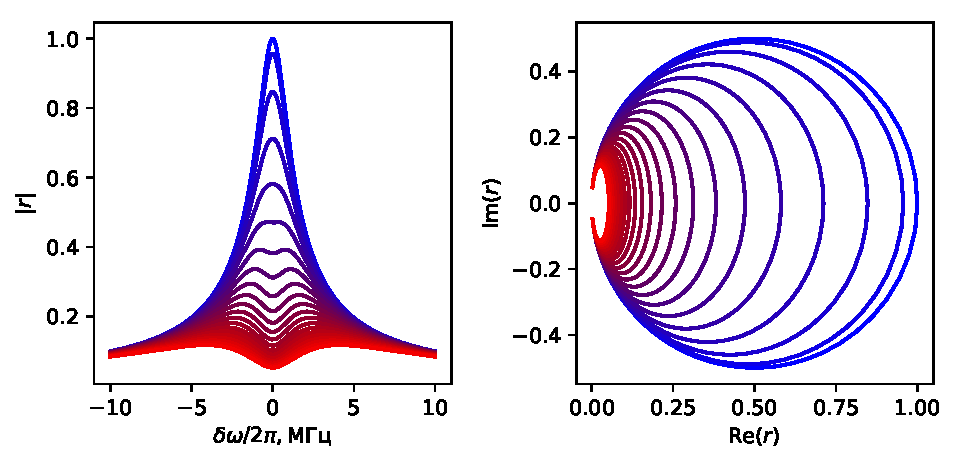
\includegraphics[width=0.9\textwidth]{relf.pdf}
	\caption[Коэффициент отражения в стационарном состоянии]{Стационарный коэффициент отражения непрерывной волны на частоте $\omega_q+\delta\omega$, направляемой на кубит. Слева: Зависимость $|r|(\delta\omega)$, где $\delta\omega/2\pi=[-10,10]$~МГц. Различные линии соответствуют значениям $\Omega/2\pi=[0,6]$~МГц, для всех линий $\Gamma_1/2\pi=2$~МГц, $\gamma_\varphi/2\pi=0$~МГц. Справа: $r$ на комплексной плоскости для $\delta\omega/2\pi=[-20,20]$~МГц и для тех же значений параметров $\Omega,\Gamma_1,\gamma_\varphi$.  }
	\label{fig: refl}
\end{figure}
\subsubsection{Спектр некогерентного излучения}
Будем рассматривать комплексный оператор напряжения в линии $\hat{V}(t)$ как некоторый случайный стационарный процесс. К нему можно применить теорему Винера-Хинчина, которая устанавливает однозначную связь между автокорреляционной функцией процесса, которую можно записать в виде $\braket{\hat{V}^{+}(0)\hat{V}^{-}(\tau)}$, и спектральной плотностью процесса. Будем искать спектральную плотность в стационарном состоянии:  
\begin{equation}
S_{VV}(\omega) = \frac{1}{2\pi Z}\int\limits_{-\infty}^{\infty}\braket{\hat{V}^{+}(0)\hat{V}^{-}(\tau)}_{ss}e^{i\omega \tau}\,d\tau
\end{equation}
С учетом \eqref{eq: refl} для оператора напряжения в точке связи с кубитом $x=0$ можно получить выражение:
\begin{equation}
\hat{V}^{\pm}(t) = i\frac{\hbar\Gamma_1}{\mu}\hat{\sigma}_\mp(t)e^{\mp i\omega_d t}.
\label {eq: sc_field}
\end{equation}
Необходимо отметить, что это выражение представляет частный случай общего результата, согласно которому, поле, излучаемое атомом в дипольном приближении на далекое расстояние, пропорционально операторам $\sigma_-$ и $\sigma_+$ (см. уравнение (10.A.16) в \cite{Scully}).
C учетом последнего равенства имеем:
\begin{equation}
S_{VV}(\omega) = \frac{\hbar\omega_q
	 \Gamma_1}{2\pi}\int\limits_{-\infty}^{\infty}\braket{\hat{\sigma}_{+}(0)\hat{\sigma}_{-}(\tau)}_{ss}e^{i(\omega-\omega_d) \tau}\,d\tau.
\label{eq: SVV_sigmas}
\end{equation}
Операторы $\hat{\sigma}_+$ и $\hat{\sigma}_-$ можно представить при помощи введения операторов флуктуаций:
\begin{equation}
\hat{\sigma}_\pm(t)=\braket{\sigma_\pm}_{ss}+\Delta\hat{\sigma}_\pm(t),
\label{eq: fluct}
\end{equation}
при этом $\braket{\Delta\hat{\sigma}_\pm(t)}_{ss}\!=\!0$ по определению. С учетом этого представления, коррелятор преобразуется следующим образом:
\begin{equation}
\braket{\hat{\sigma}_{+}(0)\hat{\sigma}_{-}(\tau)}_{ss} = \braket{\hat{\sigma}_+(0)}_{ss} \braket{\hat{\sigma}_-(\tau)}_{ss} + \braket{\Delta\hat{\sigma}_{+}(0)\Delta\hat{\sigma}_{-}(\tau)}_{ss}.
\label{eq: correlator}
\end{equation} 
Таким образом, полная спектральная плотность излучения будет складываться из эластичной и неэластичной части:
\begin{equation}
S_{VV}(\omega) = S_{el}(\omega) + S_{in}(\omega)
\end{equation}
Первое слагаемое \eqref{eq: correlator} представляет собой произведение средних значений операторов в стационарном состоянии, и может быть посчитано с использованием \eqref{eq: stat_sol}, для простоты полагая $\delta\omega\!=\!0$:
\begin{equation}
\braket{\hat{\sigma}_\pm}_{ss} = \pm \frac{ie^{\mp i\varphi}}{2}\frac{\Gamma_1\Omega}{\Gamma_1\Gamma_2+\Omega^2}
\end{equation}
С использованием этого соотношения можно посчитать когерентную (эластичную) часть спектра:
\begin{align}
S_{el}(\omega) =& \frac{\hbar\omega_q
	\Gamma_1}{2\pi}\int\limits_{-\infty}^{\infty}\braket{\hat{\sigma}_{+}(0)}_{ss}\braket{\hat{\sigma}_{-}(\tau)}_{ss}e^{i(\omega-\omega_d) \tau}\,d\tau,\\
S_{el}(\omega) =& \frac{\hbar\omega_q\Gamma_1}{4}\frac{\Gamma_1^2\Omega^2}{\left(\Gamma_1\Gamma_2+\Omega^2\right)^2}\,\delta\!\left(\omega-\omega_d\right)
\end{align}
В случае слабого поля $\Omega^2\!\ll\!\Gamma_1\Gamma_2$ и $\Gamma_2\!=\!\Gamma_1/2$ имеем $S_{el}(\omega)\!=\!\delta\!\left(\omega-\omega_d\right)\cdot\hbar \omega_q\Omega^2/\Gamma_1$.  Расчет неэластичной части спектра 
\begin{equation}
S_{in}(\omega) = \frac{\hbar\omega_q
	\Gamma_1}{2\pi}\int\limits_{-\infty}^{\infty}\braket{\Delta\hat{\sigma}_{+}(0)\Delta\hat{\sigma}_{-}(\tau)}_{ss}e^{i(\omega-\omega_d) \tau}\,d\tau.
\label{eq: inelastic}
\end{equation}
требует вычисления кореллятора флуктуаций. 

Легко понять, что зависимость $\rho(t)$, получаемая из уравнений Блоха, сама по себе не дает корелляции, представляющие собой средние по состоянию значения произведения операторов в разные моменты времени. Для этого потребуется использовать так называемую \textit{квантовую регресионную теорему}, которая позволяет найти временную зависимость коррелляторов по известной динамике матрицы плотности. Кратко проиллюстрируем суть теоремы. Рассмотрим атом, взаимодействующий с некоторым резервуаром и описываемый матрицей плотности $\rho(t)$, которую в общем случае нельзя представить в виде произведения $\rho_a(t)\otimes\rho_R(t)$, так как атом и окружение могут быть запутаны. Рассмотрим марковское приближение, согласно которому, существует некоторый нулевой момент времени, в который состояния можно факторизовать: $\rho(0)=\rho_a(0)\otimes\rho_R(0)$ Зная начальное состояние $\rho(0)$, можно найти состояние системы в произвольный момент времени при помощи оператора эволюции: $\rho(t)=U(t)\rho(0)U^\dagger(t)$. Для того чтоб выделить состояние атома в момент времени $\tau$, необходимо взять частичный след по переменным резервуара: $\rho_a(\tau) = \tr_R(\rho(\tau))$. С учетом этого можно записать выражение для среднего значения оператора $\sigma_-$ в момент времени $\tau$ может быть записано как:
\begin{align}
\braket{\hat{\sigma}_-(\tau)} &=  \tr_a\left[\hat{\sigma}_-(0)\rho_a(\tau)\right],\\ \braket{\hat{\sigma}_-(\tau)} &=\tr_a\left[\hat{\sigma}_-(0)\tr_R\left(U(\tau)\left[\rho_a(0)\otimes\rho_R(0)\right]U^\dagger(\tau)\right)\right].
\label{eq: exp}
\end{align}
Аналогичным образом запишем среднее значение коррелятора:
\begin{multline}
\braket{\hat{\sigma}_+(0)\hat{\sigma}_-(\tau)} =\tr_a\left[\hat{\sigma}_+(0)\hat{\sigma}_-(0)\tr_R\left(U(\tau)\left[\rho_a(0)\otimes\rho_R(0)\right]U^\dagger(\tau)\right)\right]=\\=\tr_a\left[\hat{\sigma}_-(0)\tr_R\left(U(\tau)\left[\rho_a(0)\hat\sigma_+(0)\otimes\rho_R(0)\right]U^\dagger(\tau)\right)\right],
\label{eq: corr}
\end{multline}
где в последнем равенстве использованы свойства частичного следа \cite{nielsen2002quantum}. Сравнивая выражения \eqref{eq: exp} и \eqref{eq: corr}, приходим к интересному выводу: для того, чтоб получить зависимость коррелятора $\braket{\hat{\sigma}_+(0)\hat{\sigma}_-(\tau)}$, достаточно использовать выражение $\braket{\hat{\sigma}_-(\tau)}$, но вместо начального состояния атома $\rho_a(0)$ необходимо подставить оператор $\rho_a(0)\hat{\sigma}_+$. Аналогичное справедливо и для оператора $\braket{\Delta\hat{\sigma}_+(0)\Delta\hat{\sigma}_-(\tau)}$. В более обобщенном смысле теорема утверждает, что если справедлива система уравнений, описывающее динамику средних некоторого полного набора операторов $\hat{A}_i$ и записываемая в векторно-матричной форме:
\begin{equation}
\frac{d\braket{\vec{A}(t)}}{dt} = \mathbf{M}\braket{\vec{A}(t)},
\end{equation}
то для произвольного оператора системы $\hat{O}(t)$ справедливо также:
\begin{equation}
\frac{d}{d\tau}\!\braket{\hat{O}(t)\vec{A}(t+\tau)} = \mathbf{M}\braket{\hat{O}(t)\vec{A}(t+\tau)}
\end{equation}
Для нахождения $\braket{\Delta\vec{\sigma}(\tau)}$ можно использовать решение уравнений Блоха \eqref{eq: Bloch}. Перепишем уравнения Блоха для нестационарной части излучения:
\begin{equation}
\braket{\Delta\dot{\vec{\sigma}}(\tau)} = \mathbf{M}\braket{\Delta\vec{\sigma}(\tau)} \rightarrow \braket{\Delta\vec{\sigma}(\tau)} = e^{\mathbf{M}\tau}\braket{\Delta\vec{\sigma}(0)} %=e^{\mathbf{M}\tau}\left(\vec{\sigma}_0-\braket{\vec{\sigma}}_{ss}\right).
\label{eq: bloch_delta}.
\end{equation}
Согласно квантовой регресионной теореме, для нахождения $\braket{\Delta\hat{\sigma}_+(0)\Delta\vec{\sigma}(\tau)}$ вместо $\braket{\Delta\vec{\sigma}(0)}$ нужно подставить в \eqref{eq: bloch_delta} начальное условие $\braket{\Delta\hat{\sigma}_+(0)\Delta\vec{\sigma}(0)}$, которое вычисляется c помощью \eqref{eq: fluct} и \eqref{eq: stat_sol} как: 
\begin{equation}
\braket{\Delta\hat{\sigma}_+(0)\Delta\vec{\sigma}(0)} = \braket{\hat{\sigma}_+\vec{\sigma}}_{ss} - \braket{\hat{\sigma}_+}_{ss}\braket{\vec{\sigma}}_{ss}=
\left[\begin{matrix}
\frac{\Omega ^2}{\Gamma_1 ^2+2 \gamma_\varphi  \Gamma_1 +2 \Omega ^2} \\
\frac{i \Omega ^2 \left(-\Gamma_1 ^2+2 \gamma_\varphi  \Gamma_1 +2 \Omega ^2\right)}{\left(\Gamma_1 ^2+2 \gamma_\varphi  \Gamma_1 +2 \Omega ^2\right)^2} \\
-\frac{2 i \Gamma_1  \Omega ^3}{\left(\Gamma_1 ^2+2 \gamma_\varphi  \Gamma_1 +2 \Omega ^2\right)^2} 
\end{matrix}\right]
\end{equation}
после чего из \eqref{eq: bloch_delta} получаем:
\begin{multline}
\braket{\Delta\hat{\sigma}_+(0)\Delta\hat{\sigma}_-(\tau)}_{ss} = \frac{\Omega ^2}{2 \left(2 \gamma_\varphi  \Gamma_1 +\Gamma_1 ^2+2
	\Omega ^2\right)} \Bigg[e^{-\frac{1}{2} t (2 \gamma_\varphi +\Gamma_1 )} + e^{-\frac{1}{4} t (2 \gamma_\varphi +3 \Gamma_1 )} \cdot \\ \cdot \left( \frac{2 \gamma_\varphi  \Gamma_1 -\Gamma_1 ^2+2 \Omega ^2}{2 \gamma_\varphi  \Gamma_1 +\Gamma_1 ^2+2
	\Omega ^2}
		\cos \Omega _g t - \frac{ 2 \Omega ^2 (2 \gamma_\varphi -5 \Gamma_1 )+\Gamma_1  (\Gamma_1 -2 \gamma_\varphi )^2}{4\Omega_g\left(2 \gamma_\varphi  \Gamma_1 +\Gamma_1 ^2+2
			\Omega ^2\right)} \sin \Omega _g  t \right)\Bigg].
\label{eq: Corr(t)}
\end{multline}
Выражение \eqref{eq: Corr(t)} получено без каких-либо приближений. Дальнейшее вычисление спектральной плотности сводится к преобразованию Фурье и приводит к достаточно громоздким выражениям, поэтому оно будет опущено. Для частного случая сильного драйва $4\Omega \gg \Gamma_1, \gamma_\varphi$ получается выражение:
\begin{equation}
S_{in}(\delta\omega) = \frac{1}{2\pi}\frac{\hbar \omega_q\Gamma_1}{4}\Big(\frac{\gamma_s}{(\delta\omega+\Omega)^2+\gamma_s^2}+\frac{2\gamma_c}{\delta\omega^2+\gamma_c^2}+\frac{\gamma_s}{(\delta\omega-\Omega)^2+\gamma_s^2}\Big),
\label{eq: mollow}
\end{equation}
где введены обозначения $\gamma_c = \Gamma_1/2 + \gamma_\varphi = \Gamma_2$, $\gamma_s = 3\Gamma_1/4 + \gamma_\varphi/4 = (\Gamma_1 + \Gamma_2)/2$.
Отличительной особенностью данного спектра явяется наличие боковых пиков при $\delta\omega = \pm \Omega$. Отметим также, что в отличие от спектральной плотности эластичной части излучения, которая максимальна при $\Omega = \sqrt{\Gamma_1 \Gamma_2}$ и далее уменьшается при увеличении $\Omega$, спектральная плотность неэластичной части возрастает от нуля при $\Omega = 0 $ до некоторого максимального значения. Поскольку спектр \eqref{eq: mollow} состоит из трех лоренцевских пиков, достаточно разделяющихся при $\Omega \gg \Gamma_1$, то полная мощность, рассеиваемая кубитом, равна $\hbar \omega_q \Gamma_1/2$. Этот ответ допускает наглядную качественную интерпретацию. Сильное поле не взаимодействует с кубитом когерентно, но вызывает квантово-механические скачки с основного на возбужденный уровень и обратно со средней частотой $\Gamma_1$. Таким образом, эффективно кубит излучает мощность, соответствующую половине энергии фотона, которая излучается за время релаксации. Спектр некогерентного излучения изображен на Рис.~\ref{fig: Mollow}.
\begin{figure}[th]
	\centering
	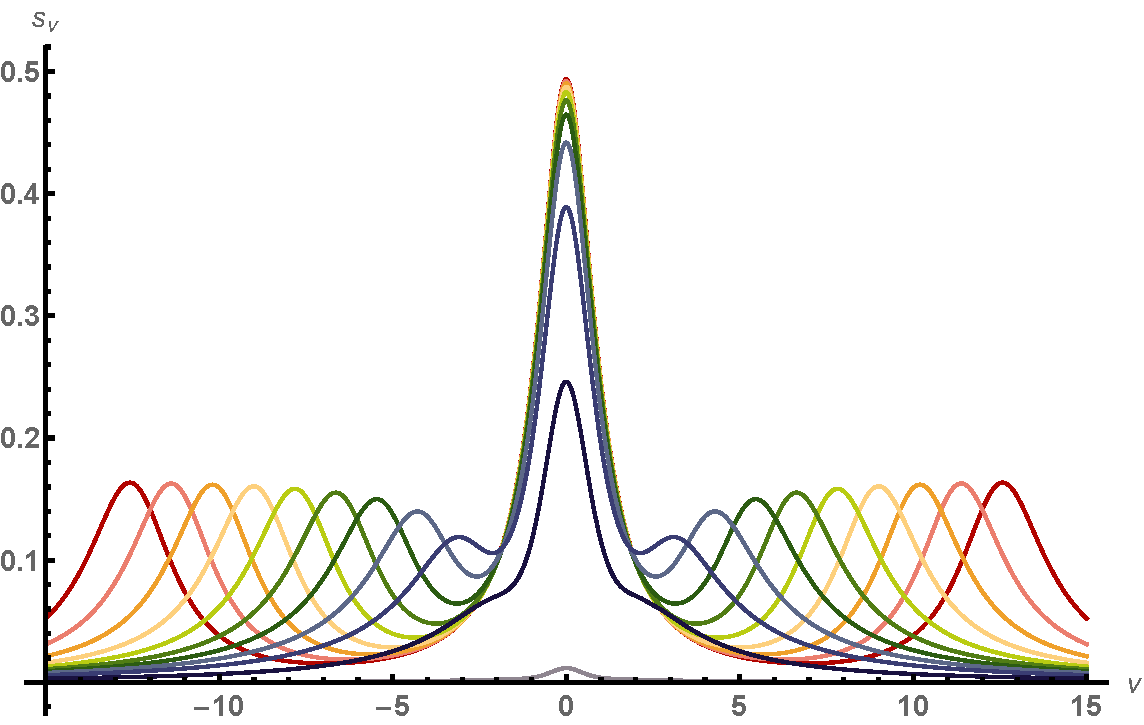
\includegraphics[width=0.7\textwidth]{images/Mollow.pdf}
	\caption[Спектр резонансной флуоресценции.]{Спектр неэластичного рассеяния для $\Gamma_1 = 2$ МГц, $\gamma_\varphi=0$, $\Omega = [1.5, 12.5]$~МГц. }
	\label{fig: Mollow}
\end{figure}
%где в последнем равенстве использовано начальное условие $\vec{\sigma}_0 = \{0,0,\!-\!1\}$. В результате искомый кореллятор находится как
%\begin{equation}
%\braket{\Delta\hat{\sigma}_-(0)\Delta\hat{\sigma}_+(0)} = \frac{1}{2} \left(e^{-\frac{1}{2} \tau (2 \gamma +\Gamma )}+\frac{\Omega _g e^{-\frac{1}{4} \tau (2 \gamma +3 \Gamma )} \left(\left(4 \gamma ^2
%	\Gamma -i \Gamma  \Omega  (6 \gamma +\Gamma )+4 \gamma  \Omega ^2-\Gamma ^3\right) \sinh \left(t \Omega _g \right)-4 \Omega _g \left(2 \gamma  \Gamma
%	+\Gamma ^2-i \Gamma  \Omega +2 \Omega ^2\right) \cosh \left(t \Omega _g \right)\right)}{4 \Gamma  (2 \gamma +\Gamma )+8 \Omega ^2}\right)
%\end{equation}

Мы рассмотрели основные эффекты, возникающие при взаимодействии двухуровневой системы (сверхпроводникового кубита), сильно связанной с волноводом, и внешнего классического поля, распространяющегося в волноводе (проходной линии). Можно отметить, что даже в таком простом случае физика происходящих явлений весьма нетривиальна. Однако, в главе \ref{ch: Quant} показано, что сверхпроводниковые кубиты не являются двухуровневыми системами: во многих случаях необходимо учитывать третий и следующие уровни энергии. В квантовой оптике, взаимодействие света с трехуровневой системой порождает целый ряд явлений, таких как электромагнитно-индуцированная прозрачность, когерентный захват заселенности и другие. Опишем некоторые из эффектов, возникающие в трехуровневых системах.

\subsection{Квантовооптические эффекты в трёхуровневых системах}
\label{sec: qo3ls}
СКЦ, как и любая квантовая система, имеет большое количество собственных энергетических уровней. Если энергии третьего (второго возбужденного) уровня СКЦ настолько велики, что частоты переходов с первых двух уровней превышают частоты внешнего электромагнитного поля, с которым взаимодействует система, то справедливо двухуровневое приближение. Однако во многих случаях это не так, и необходимо учитывать наличие третьего уровня. 

Как и для <<природных>> атомов химических элементов, для сверхпроводниковых цепей справедливы правила отбора: в дипольном приближении, запрещены переходы между теми состояниями, волновые функции которых имеют одинаковую симметрию. Так, например, для трансмонов, структура волновых функций которых достаточно близка к гармоническому осциллятору, запрещены переходы $\ket{0}\rightarrow\ket{2}$ и обратно. На основе правил отбора можно выделить несколько типов трехуровневых систем, схематично изображенных на Рис.~\ref{fig: 3LS_class}.  
\begin{figure}[th]
	\centering
	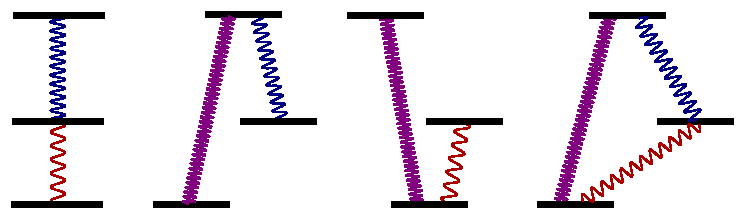
\includegraphics[width=0.8\textwidth]{images/3Ls_V_Lbd_ladder.pdf}
	\caption[Классификация трехуровневых систем по разрешенности переходов.]{Классификация трехуровневых систем, порождаемая правилами отбора; слева направо --- схематичное изображение $\Xi$-, $\Lambda$-, $V$-, и $\Delta$-системы, соответственно. Волнистые линии связывают пары уровней, переход между которыми разрешен в дипольном приближении.}
	\label{fig: 3LS_class}
\end{figure}
Конфигурации уровней под названием $\Xi$-система (или лестничная система), $\Lambda$-система и $V$-система часто возникают в природных атомах, тогда как $\Delta$-система достаточно нехарактерна для них и поэтому достаточно слабо изучена экспериментально. Она может быть реализована только при помощи киральных молекул, а также в искусственных оптических системах на основе СКЦ. 
\subsubsection{Электромагнитно-индуцированная прозрачность и расщепление Аутлера-Таунса}\label{AT}
Рассмотрим эффекты, связанные с наличием двух электромагнитных полей, взаимодействующих с трехуровневой системой. По аналогии с двухуровневой системой, можно записать гамильтониан, описывающий $\Lambda$-систему с частотами переходов $\omega_{02}$~и~$\omega_{12}$, которая взаимодействует с двумя электромагнитными модами $\omega^d_{12}$~и~$\omega^d_{02}$:
\begin{equation}
H = \left[\begin{matrix}\delta_{02} - \omega^{d}_{02} & 0 & \Omega_{02} \cos{\omega^{d}_{02} t }\\0 & \delta_{12} - \omega^{d}_{12} & \Omega_{12} \cos{\omega^{d}_{12} t }\\\Omega_{02} \cos{\omega^{d}_{02} t } & \Omega_{12} \cos{\omega^{d}_{12} t } & 0\end{matrix}\right],
\end{equation}
где введено обозначение $\delta_{12} = \omega^d_{12}-\omega_{12}$, $\delta_{02}$ --- аналогично. Переходя во вращающуюся систему отсчета и используя приближения вращающейся волны, этот гамильтониан можно привести к виду:
\begin{equation}
H_{RW\!A}=\left[\begin{matrix}\delta_{02} & 0 & \frac{\Omega_{02}}{2}\\0 & \delta_{12} & \frac{\Omega_{12}}{2}\\\frac{\Omega_{02}}{2} & \frac{\Omega_{12}}{2} & 0\end{matrix}\right]
\label{eq: 3LS_Hrwa}
\end{equation}
\begin{figure}[h]
	\centering
	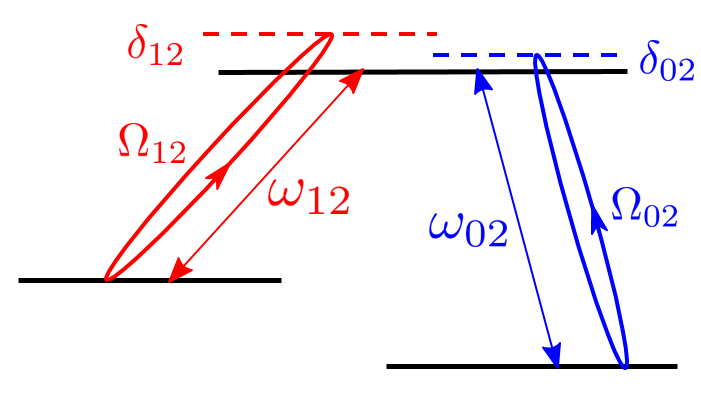
\includegraphics[width=0.5\textwidth]{images/ATS.png}
	\caption[Схема возбуждения $\Lambda$-системы электромагнитным полем]{Схема трехуровневой $\Lambda$-системы под действием двух непрерывных волн с частотами $\omega^d_{i2} = \omega_{i2}+\delta_{i2}, i={0,1}$, возбуждающих переходы в системе. }
	\label{img: Lambda}
\end{figure}
Оператор плотности, описывающий трехуровневую систему, можно записать стандарным образом:
\begin{equation}
\rho = \left[\begin{matrix}- \rho_{11} - \rho_{22} + 1 & i \rho^{i}_{01} + \rho^{r}_{01} & i \rho^{i}_{02} + \rho^{r}_{02}\\- i \rho^{i}_{01} + \rho^{r}_{01} & \rho_{11} & i \rho^{i}_{12} + \rho^{r}_{12}\\- i \rho^{i}_{02} + \rho^{r}_{02} & - i \rho^{i}_{12} + \rho^{r}_{12} & \rho_{22}\end{matrix}\right]
\end{equation}
Влияние диссипации и декогеренции на динамику системы описывается стандартным образом, см. \ref{sec:Lind}; отметим, что в трехуровневой системе скорости релаксации $ \Gamma_{01}, \Gamma_{02}, \Gamma_{12}$ и дефазировки $\gamma_{02}, \gamma_{12}$~и~$\gamma_{01}$ в общем случае независимы и могут значительно отличаться. Линдбладовский член имеет следующий вид:
\begin{equation}
\left[\begin{matrix}\Gamma_{02} r_{22} & - \gamma_{01} \left(i r^{i}_{01} + r^{r}_{01}\right) & - \frac{\left(i r^{i}_{02} + r^{r}_{02}\right) \left(\Gamma_{02} + \Gamma_{12} + 2\gamma_{02}\right)}{2}\\ \gamma_{01} \left(i r^{i}_{01} - r^{r}_{01}\right) & \Gamma_{12} r_{22} & - \frac{\left(i r^{i}_{12} + r^{r}_{12}\right) \left(\Gamma_{02} + \Gamma_{12} + 2\gamma_{12}\right)}{2}\\\frac{\left(i r^{i}_{02} - r^{r}_{02}\right) \left(\Gamma_{02} + \Gamma_{12} + 2\gamma_{02}\right)}{2} & \frac{\left(i r^{i}_{12} - r^{r}_{12}\right) \left(\Gamma_{02} + \Gamma_{12} + 2\gamma_{12}\right)}{2} & - r_{22} \left(\Gamma_{02} + \Gamma_{12}\right)\end{matrix}\right]
\label{eq: Lindblad_3ls}
\end{equation}

Рассмотрим случай, когда амплитуда $\Omega_{12}$ достаточно большая по сравнению со всеми константами релаксации и дефазировки и $\delta_{12}=0$. Это поле будет связывать состояния $\ket{1}$ и $\ket{2}$, и формировать новые собственные состояния системы ---  так называемые \textit{одетые состояния} $\left(\ket{1} \pm \ket{2}\right)/\sqrt{2}$ c энергиями $\pm\Omega_{12}/2$. Обозначим $\delta_{02}=\delta$. Предположим теперь, что амплитуда поля $\Omega_{02}$ невелика, и поле носит характер пробного сигнала, не меняя при этом структуру уровней системы. Как мы увидим далее, это пробное поле позволяет визуализировать одетые уровни, созданные сильной накачкой перехода 1-2. Для нахождения стационарного состояния системы необходимо решить уравнение \eqref{eq: QLiouv} с гамильтонианом \eqref{eq: 3LS_Hrwa},  диссипатором \eqref{eq: Lindblad_3ls}, а также зануленной левой частью. В полной аналогии с двухуровневой системой можно показать, что если известно стационарное состояние, то коэффициент отражения для поля, рассеянное на пробной частоте $\omega^d_{02}$, имеет вид:
\begin{equation}
r_{02} = i\frac{\Gamma_{02}}{\Omega_{02}}\braket{\hat{\sigma}_{02}}_{ss}e^{i\omega^d_{02}t}, 
\end{equation}
ср. с \eqref{eq: refl}. График зависимости $\text{Re}\left({r_{02}}(\delta)\right)$ для различных значений амплитуды драйва $\Omega_{12}$, представленный на Рис.~\ref{img: EIT_ATS}, наглядно иллюстрирует возникновение одетых состояний. 
\begin{figure}[ht]
	\centering
	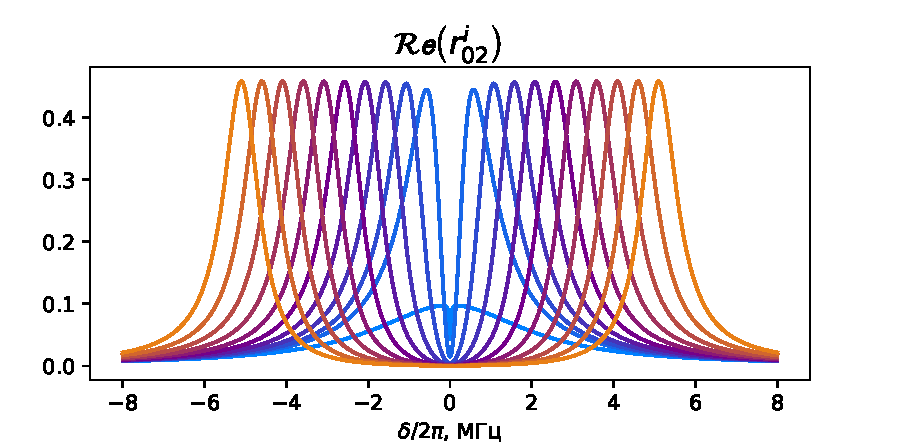
\includegraphics[width=0.9\textwidth]{images/EIT_ATS_plot.pdf}	 
	\caption[Электромагнитно индуцированная прозрачность и расщепление Аутлера-Таунса в $\Lambda$-системе]{Коэффициент отражения пробного поля  амплитудой $\Omega_{02}=50$~кГц в зависимости от отстройки $\delta_{02}=\delta.$ Амплитуда поля накачки $\Omega_{12} = [0.1, 5.1]$~МГц, $\Gamma_{01}=0, \gamma_{12}=\gamma_{02}=\gamma_{01}=0.1$~МГц,  $\Gamma_{02}=\Gamma_{12}=2$~МГц. При малых амплитудах наблюдается провал, соотвествующий электрромагнитно-индуцированной прозрачности, а при больших формируются два пика, образующие расщепление Аутлера-Таунса.}
	\label{img: EIT_ATS}
\end{figure}
При $\Omega_{12} \gg \Gamma_{12}, \Gamma_{02}$ рассеянное поле имеет два максимума лоренцевской формы при $\delta = \pm \Omega_{12}/2$. Этот эффект называют расщеплением Аутлера-Таунcа. Отметим также случай слабого драйва, соответствующий $2\Omega_{12}<\Gamma_{02}+\gamma_{02}-\gamma_{01}$. В этом случае рассеянное поле представляется в виде одиночного лоренцевского пика, однако, при $\delta=0$ наблюдается достаточно узкий провал, достигающий нуля при $\gamma_{01}=0$. Это явление называется электромагнитно-индуцированной прозрачностью. Можно показать, что в этом случае провал возникает за счет деструктивной интерференции между полем накачки и пробным полем, тогда как при расщеплении Аутлера-Таунса происходит сдвиг резонансных частот одетых уровней за счет более сильного драйва.
Точная формула, описывающая рассмотренные эффекты, достаточно громоздка, но может быть записана приближенно, если пренебречь чистой дефазировкой и разложить точное выражение в ряд по амплитуде пробного поля $\Omega_{02}$:
\begin{equation}
\text{Re}\left(r_{02}\right)\approx -\frac{4 \left(\Gamma _{12}+\Gamma _{02}\right) \delta ^2 \Omega_{02}}{4 \delta ^2 \left(\left(\Gamma _{12}+\Gamma _{02}\right){}^2+4 \delta^2\right)-8
	\delta ^2 \Omega_{12} ^2+\Omega_{12} ^4}
\end{equation}
Электромагнитно-индуцированная прозрачность и расщепление Аутлера-Таунса были хорошо изучены в рамках квантовой оптики видимого диапазона на природных атомах \cite{Boller_EIT,picque1976direct}. Однако, эти эффекты неоднократно продемонстрированы и в рамках микроволновой квантовой оптики на СКЦ, включая как трансмоны, так и потоковые кубиты \cite{Abdumalikov_EIT, Baur, ATS_3LS, li2012dynamical,ATS_3D_transmon}. 

\subsubsection{Когерентный захват заселенности}
Еще один интересный эффект --- когерентный захват заселенности --- возникает в случае установления равновесия в системе при условии, что амплитуды обоих полей $\Omega_{02}$~и~$\Omega_{12}$ много больше остальных констант в системе. Будем считать, что $\delta_{12}=\delta_{02}=\delta$. В этом случае, собственные векторы гамильтониана можно выразить следующим образом:
\begin{equation}
\begin{aligned}
\ket{\psi_D} &= \cos\Phi\ket{0} - \sin\Phi\ket{1}, \\
\ket{\psi_+} &= \sin\Theta\sin\Phi \ket{0} + \cos\Theta \sin \Phi\ket{1} -\cos\Phi \ket{2}, \\
\ket{\psi_-} &= \cos\Theta\sin\Phi\ket{0} + \cos\Theta\cos\Phi\ket{1} + \sin\Phi\ket{2}.
\end{aligned}
\end{equation}
Используемые параметры $\Phi$ и $\Theta$ определяются соотношениями:
\begin{equation}
\begin{aligned}
\Omega_{02} &= A\sin 2\Phi\sin\Theta, \\
\Omega_{12} &= A\sin 2\Phi \cos\Theta, \\
\delta &= A\cos 2\Phi. 
\end{aligned}
\end{equation}
Заметим, что состояние $\ket{\phi_D}$ представляет из себя суперпозицию состояний, каждое из которых не подвергается радиационному распаду в случае $\Lambda$-системы. Такое состояние называется \textit{темным}. Если приготовить темное состояние, то его распад будет определяться неизлучательными процессами, и следовательно, может быть на порядки медленнее распада состояния $\ket{2}$, сопровождающегося излучением фотонов.
\begin{figure}[h]
	\centering
	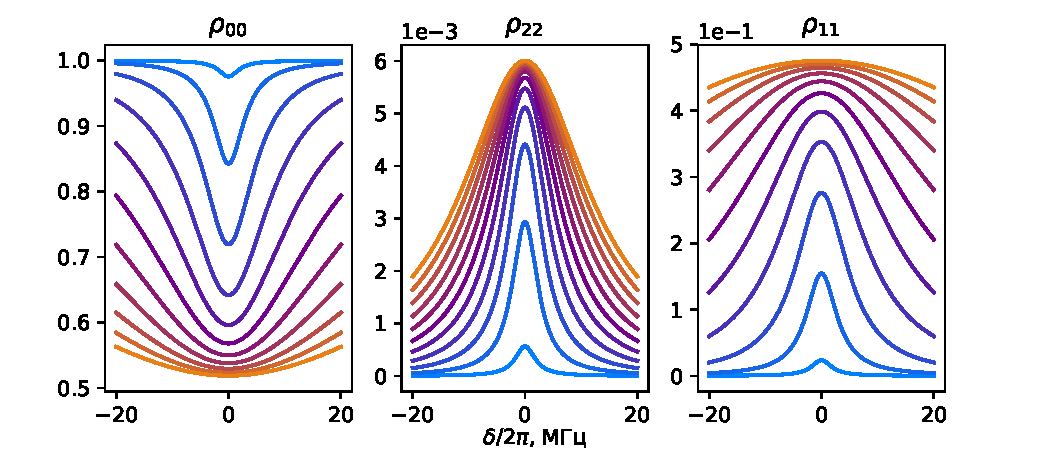
\includegraphics[width=0.95\textwidth]{images/CPT_plot_small.pdf}	 
	\caption[Когерентный захват заселенности в $\Lambda$-системе]{Диагональные элементы матрицы плотности стационарного состояния $\Lambda$-системы в зависимости от отстройки $\delta$. Кривые построены при $\Gamma_{01}/2\pi=\Gamma_{12}/2\pi = 2$~МГц, $\Gamma_{01}/2\pi=50$~кГц, амплитуды драйва меняются для различных кривых в пределах $\Omega_{01}/2\pi=\Omega_{12}/2\pi = [0.1, 2.1]$~МГц.}
	\label{img: CPT_plot}
\end{figure}
Другими словами, темное состояние метастабильно и может служить перспективным инструментом для реализации квантовой памяти. Эффективный способ заселить это состояние - обеспечить достаточно сильную накачку системы на частотах разрешенных переходов. Диагональные элементы матрицы плотности стационарного состояния представлено на рисунке \ref{img: CPT_plot}. Поскольку всегда существует некоторая ненулевая релаксация $\Gamma_{01}$, то при слабой амплитуде драйва система практически не выходит из основного состояние $\ket{0}$. Однако, по мере увеличения амплитуд заселенность уровней $\ket{0}$ и $\ket{1}$ практически выравнивается, и состояние системы стремится к $\left(\ket{0}+\ket{1}\right)/\sqrt{2}$, при этом уровень $\ket{2}$ остается пустым. Модуль недиагональных элементов $\rho_{01}$~и~$\rho_{10}$ также стремится к $0.5$, что означает высокую когерентность стационарного состояния --- поэтому эффект и называется когерентным захватом заселенности. Фаза стационарной суперпозиции определяется относительной фазой сигналов накачки. 


Завершая обзор трехуровневых искусственных атомов, можно отметить, что по мере усложнения системы возникает множество различных явлений, по-разному проявляющих себя в эксперименте и представляющих большой интерес в качестве как фундаментальных явлений квантовой оптики, так и основы для будущих квантовых сверхпроводниковых оптических устройств. 

\subsection{Обзор достижений микроволновой квантовой оптики в волноводе}
В дополнение к изложенному приведем обзор некоторых важных результатов квантовой оптики и фотоники на СКЦ. Поскольку эта область уже достаточно обширна, то сфокусируемся более узко на экспериментах, изучающих взаимодействие атома с континуумом мод в волноводе или в копланарной линии. Обнаружение резонансной флуоресценции от сверхпроводникового потокового кубита \cite{Astafiev2010resonance} --- первый эксперимент, который пробудил интерес к волноводной квантовой электродинамике. В первую очередь, это обусловлено высокой эффективностью, превышающей 94\% в пионерском эксперименте и 99\% в последующих исследованиях \cite{single-photon-router,Delsing-giant-Kross-Kerr}, притом это улучшение практически не потребовало изменения архитектуры и было связано с улучшением качества кубита. Эффективность связи хорошо характеризуется долей отраженной мощности (power extinction) в режиме слабого когерентного сигнала, не насыщающего атом. Кроме сверхпроводящих кубитов, волноводная квантовая электродинамика реализовывалась и на других физических системах: квантовые точки, связанные с плазмонными волноводами \cite{akimov2007generation,martin2010resonance}, либо же естественные атомы, связываемые с оптическим волокном \cite{Vetsch2010,Goban2012fibertrap}. Оба этих подхода страдают как от недостаточного совмещения электромагнитных мод, так и от значительной безызлучательной релаксации. Для квантовых точек эффективность связи в среднем достигает 60\%, хотя отдельные работы сообщают о значениях более 90\% \cite{Arcari2014NearUnity}. Для естественных атомов доля отраженной мощности не превышает 12\% \cite{tey2008strong-int,Gerhard2007moleculeExt}. Этот факт делает сверхпроводниковые кубиты наиболее многообещающей платформой для изучения волноводной квантовой оптики.

После обнаружения резонансной флуоресценции, были воспроизведен целый ряд фундаментальных квантовооптических эффектов, известных ранее по изучению других физических систем. Подробно изучалась временная динамика кубита под воздействием поля в линии \cite{abdumalikov2011dynamics}. Демонстрация особенностей неэластичного спектра резонансной флуоресценции под действием сжатого вакуума \cite{Toyli2016ResSqueez} впервые подтвердила соответствующие расчеты \cite{CarmichaelSqueezedFluor}, сделанные в конце 80-х годов. Проведен ряд экспериментов с кубитом в качестве трехуровневой системы, например, изучена электромагнитно-индуцированная прозрачность \cite{Abdumalikov_EIT}, показан эффект кросс-керровского фазового сдвига \cite[]{Delsing-giant-Kross-Kerr} при расщеплении Аутлера-Таунса, которе также было подробно изучено в случае трехуровневого кубита-трансмона \cite[]{ATS_3LS,ATS_3D_transmon,Baur} и также для фазового кубита \cite{li2012dynamical}. Использование третьего уровня потокового кубита позволило получить принципиально новые результаты, например, исследовать работу кубита в качесте элементарного квантового усилителя \cite[]{Astafiev-quantum-amplifier}. Также исследовалось излучение кубита в полубесконечную линию, в том числе влияние граничных условий на скорость релаксации кубита - эффект <<сверхпроводящего зеркала>> \cite[]{hoi2015probing}.   

Отдельно следует сказать об операциях с одиночными фотонами, осуществляемых при помощи кубитов в линии --- микроволновой фотонике. За счет сильной связи с излучением и высокой нелинейности, кубит в линии имеет большой потенциал как в качестве активного элемента, так и в качестве медиатора взаимодействия различных световых мод \cite[]{Strongly1D}. Значительный прогресс в развитии микроволновой фотоники был обеспечен созданием однофотонных излучателей на основе кубита, несимметрично связанного с двумя полубесконечными линиями \cite{peng2016tuneable,Shaped_SPS,Pechal2016switch,ZhouHighEfficiency}. В дальнейшем реализована генерация фотонов с произвольной огибающей,  что предусматривает быструю перестройку связи при помощи изменения граничных условий в месте соединения кубита с полубесконечной линией \cite[]{Shaped_SPS}, либо при помощи стимулирования рамановских переходов в системе кубит-резонатор \cite{PechalShaped}. Детектирование одиночных микроволновых фотонов представляет собой значительно более сложную задачу и пока не реализовано на прикладном уровне, хотя и здесь имеются интересные теоретические предложения \cite{grimsmo2020quantum} и отдельные достаточно успешные результаты \cite{kono2018quantum,BesseQNDphoton}. Однако, показанные подходы к детектированию одиночных фотонов при помощи достаточно сложных и громоздких систем, вовлекающих в себя кубиты и резонаторы. Большую роль сыграли работы по созданию и реализации интерференционных схем с линейными детекторами \cite{daSilvaSchemes}, позволяющих провести измерение корреляционной функции $g^{(2)}(\tau)$ на входе и на выходе линии с кубитом \cite{hoi2012generation}, в ходе которых наблюдалась группировка фотонов в проходящем излучении и антигруппировка в отраженном излучении. Эта техника позволила продемонстрировать эффект Хонга-Оу-Мандела на микроволновых фотонах \cite{lang2013correlations}, реализовать генерацию и детектирование запутанных фотонов в каскадном процессе релаксации трехуровневого трансмона (являющегося $\Xi$-системой) \cite{Wallraff_entangledPhotons}, а также проводить подробную томографию фотонного состояния света в волноводе \cite{EichlerTomography}. Дальнейшее развитие подобных методик позволило также запутать кубиты на расстоянии при помощи контролируемого испускания и поглощения одиночного микроволнового фотона \cite[]{kurpiers2018deterministic}.

Большой интерес вызыват также связывание кубитов через открытый волновод, поскольку результаты, получаемые в этой сфере, могут привести к созданию принципиально новой платформы, которая будет сочетать в себе как эффективность и простоту логических операций, характерную для сверхпроводниковых кубитов в резонаторах, так и возможность передачи квантовых состояний через волноводы, характерную для линейной квантовой оптики на оптических фотонах \cite{LOQCreview}. Принципиальная возможность связывания двух кубитов посредством виртуальных фотонов, распространяющихся в волноводе, впервые теоретически исследована и реализована группой под руководством А. Вальраффа в университете Цюриха \cite{vanLoo1494}. При размещении пары кубитов с силой связи $\Gamma_1$ в волноводе на различных оптических расстояниях $d$ друг от друга проявляются различные явления: при $d \approx \lambda/2$ наблюдается сверхизлучение, когда система излучает со скоростью $\Gamma_B = 2\Gamma_1$ (см. также \cite{mlynek2014observation}), а при $d\approx 3\lambda/4$ проявляется связь между кубитами при помощи обмена виртуальных фотонов на всех частотах, кроме резонансной; максимальное значение этой связи ограничено релаксацией: $J_{max}=\Gamma_1/2$. Взаимодействие, возникающее при обмене виртуальными фотонами, достаточно сильно влияет на прохождение волновода на низкой и средней мощности сигнала, что проявляется в несиметричном прохождении излучения через волновод с двумя связанными кубитами. Более того, при $d \approx \lambda/2$ темные состояния, формируемые парой атомов, образуют нелинейную резонаторную моду \cite{mirhosseini2019cavity}, которая может связываться уже с другими кубитами в волноводе, расположенными в пучностях электрического поля в атомной моде.  Были показаны вакуумные Раби-осцилляции между пробным кубитом и атомной резонаторной модой, кроме того, изучалась структура различных темных состояний резонатора. В этом контексте особенно перспективна концепция т.н. гигантских атомов - сверхпроводниковых кубитов, которые связываются с разными точками волновода, отстоящими друг от друга на расстояние, сравнимое с длиной волны \cite{kockum2019quantum}. Для естественных атомов это принципиально невозможно, поскольку имеется природное ограничение, согласно которому длины волн на разонансных частотах атомных переходов примерно в $10^4$ раз превышают размеры атома. Выбор положения точек связи и силы взаимодействия позволяет более свободно регулировать как распад, так и взаимодействие между гигантискими атомами. С помощью связывания гигантских атомов через волновод впервые удалось реализовать двухкубитную операцию iSWAP без использования резонатора \cite[]{kannan2019waveguide} . 

В данной диссертационной работе развивается еще одно перспективное, но недостаточно изученное направление - использование кубита в качестве квантового смесителя \cite[]{vakbib1,vakbib3,vakbib4}. Смеситель является одним из основных элементов СВЧ-цепей самого различного назначения, и логично ожидать, что кубит, являясь квантовым нелинейным элементом, находящимся в волноводе с распространяющимся микроволновым излучением, может проявить интересные свойства при рассеивании этого излучения. Простейшим методом анализа смесителей является спектральный анализ, и в случае с квантовым смесителем можно ожидать появления необычных спектральных особенностей в переотраженном сигнале.
Высокая нелинейность к полям с амплитудами на уровне одиночных фотонов, относительная простота детектирования выходящего из волновода излучения и наличие однофотонных источников - все эти факторы позволяют ожидать достаточно быстрый прогресс в исследовании взаимодействия микроволновых мод на кубитах в волноводе.